% !TeX program = xelatex
\documentclass[aspectratio=1610]{beamer}
\hbadness=10000
\vbadness=10000
\hfuzz=20pt
\vfuzz=20pt
\makeatletter
\def\input@path{{notes/presentation/}{./}{}}
\makeatother
\graphicspath{{notes/presentation/}{notes/presentation/pics/}{notes/presentation/pictures/}{./}{pics/}{pictures/}}

\usetheme{wildcat}
\usepackage{beamercolorthemewildcat}
\usepackage{beamerfontthemewildcat}
\usepackage{beamerinnerthemewildcat}
\usepackage{beamerouterthemewildcat}
\usepackage{beamerthemewildcat}
\usepackage{booktabs}
\usepackage{tabularx}
\usepackage{array}
\usepackage{multirow}
\usepackage{url}
\usepackage{xcolor}
\usepackage{tikz}
\usetikzlibrary{arrows.meta,positioning,fit,shapes.geometric,calc,decorations.pathreplacing,patterns}

\setbeamertemplate{navigation symbols}{}
\setbeamertemplate{section in toc}[sections numbered]
\providecommand{\HUGE}{\Huge}

\definecolor{pureblue}{RGB}{32,76,154}
\definecolor{puregreen}{RGB}{34,139,92}
\definecolor{pureorange}{RGB}{225,123,38}
\definecolor{puregray}{RGB}{245,247,250}
\definecolor{purered}{RGB}{190,64,64}
\definecolor{purepurple}{RGB}{128,70,160}
\pdfstringdefDisableCommands{%
  \def\textbf#1{#1}%
  \def\texttt#1{#1}%
  \def\\{ }%
  \def\quad{ }%
}

\newcommand{\slidebody}{\small}
\newcommand{\slidesmall}{\footnotesize}
\newcommand{\tablesize}{\scriptsize}
\newcommand{\source}[1]{\par\vspace{0.08em}{\centering\tiny\color{black!70}Source: #1\par}}
\newcommand{\metric}[2]{\textbf{#1}\hfill #2}
\newcommand{\triplet}[3]{(#1, #2, #3)}
\newcommand{\figcaption}[1]{\vspace{0.2em}{\scriptsize\color{black!70}Figure: #1}}
\newcommand{\tabcaption}[1]{\vspace{0.2em}{\scriptsize\color{black!70}Table: #1}}
\newfontfamily\vietnamfont{DejaVu Sans}

\setbeamerfont{title}{size=\Large}
\setbeamerfont{subtitle}{family=\CamptonLight, size=\large}
\setbeamerfont{frametitle}{size=\LARGE}
\setbeamerfont{section}{family=\CamptonMedium, size=\LARGE}
\setbeamerfont{author}{size=\footnotesize}
\setbeamerfont{date}{size=\normalsize}
\setbeamerfont{institute}{size=\large}

\title{Retrieving People and Objects from Textual Descriptions via Multimodal Learning}
\subtitle{HK252-DATN-160 - Capstone Project}
\author[Nguyen Tran Dong and Le Anh Khoa]{%
Committee 6A Computer Science\\[0.18em]
Supervisor: Dr. Le Thanh Sach\\[0.18em]
Reviewer: Dr. Tran Tuan Anh\\[0.18em]
Students: Nguyen Tran Dong (2210777), Le Anh Khoa (2211595)
}
\date{}
\titlegraphic{
\includegraphics[height=2.25cm]{hcmut.png}}

\begin{document}

\begin{frame}
\titlepage
\end{frame}

\begin{frame}{Table of Contents}
\footnotesize
\tableofcontents
\end{frame}


% =============================================================================
\section{Introduction}
\subsection{Motivation, Problem, and Scope}


\begin{frame}[shrink=8]{Motivation: Relation-Aware Understanding}
\slidebody
Text-based image retrieval becomes difficult when the query describes \textbf{relations}, not only object categories.

\begin{talert}{Application value}
\begin{itemize}
  \item Relation triplets such as \triplet{person}{riding}{horse} support retrieval/localization from natural-language descriptions.
  \item Applications include security search, robot commands, AR guidance, and e-commerce search.
\end{itemize}
\end{talert}

\begin{talert}{Technical challenges}
\begin{itemize}
  \item Directional relation semantics, dense visual occlusions, fine-grained grounding, and hallucinations.
  \item Long-tailed predicate imbalance, hidden rare-relation failures, and out-of-distribution.
\end{itemize}
\end{talert}

\begin{talert}{Community context}
\begin{itemize}
  \item Recent CVPR/ICCV work keeps pushing SGG toward debiasing, query-based decoding, and open-vocabulary prediction.
  \item Standard datasets such as Visual Genome make protocol-compatible comparison possible.
\end{itemize}
\end{talert}

\source{Application and protocol context: \href{https://link.springer.com/article/10.1007/s11263-016-0981-7}{Visual Genome}, \href{https://openaccess.thecvf.com/content_cvpr_2018/html/Zellers_Neural_Motifs_Scene_CVPR_2018_paper.html}{Neural Motifs}, \href{https://openaccess.thecvf.com/content_cvpr_2020/html/Tang_Unbiased_Scene_Graph_Generation_From_Biased_Training_CVPR_2020_paper.html}{TDE}.}
\end{frame}

\begin{frame}[shrink=6]{Scene Graph Generation}
\slidebody
\begin{talert}{Task formulation}
\textbf{Input:} image $I$, object boxes $B=\{b_i\}_{i=1}^{N}$, and labels $O=\{o_i\}_{i=1}^{N}$ in PredCls.

\textbf{Output:} ranked directed triplets
\[
\mathcal{G}(I)=\{(s_i,p_{ij},o_j,\sigma_{ij})\mid i\ne j\}.
\]
\vspace{0.15em}
\centering
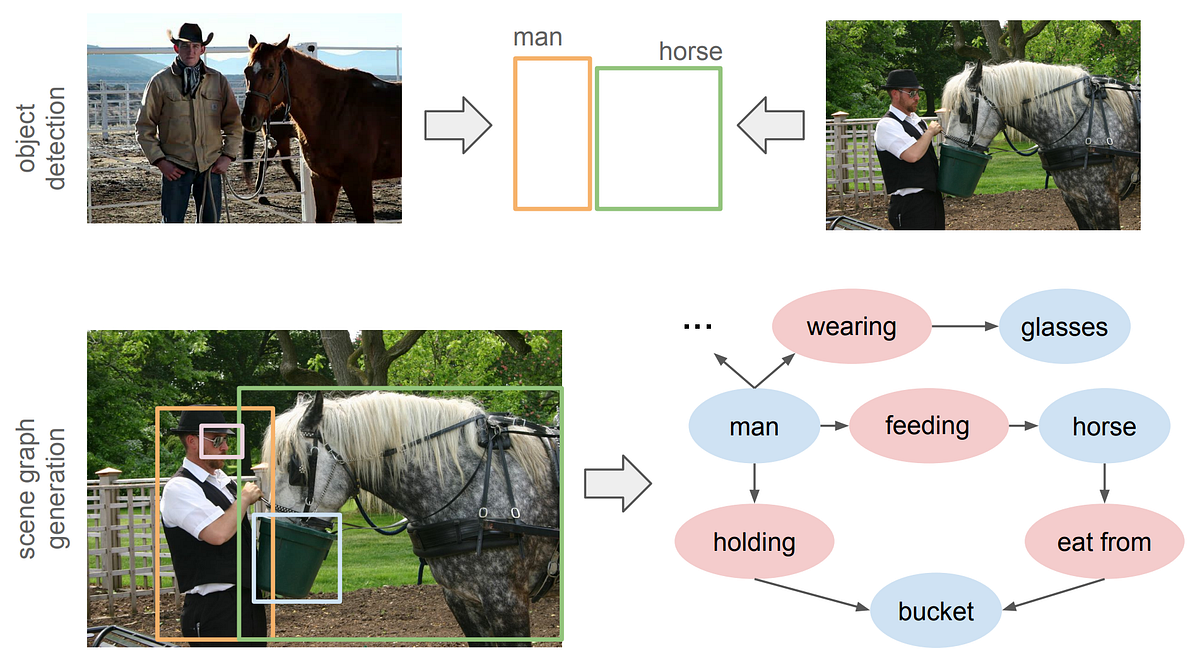
\includegraphics[width=0.86\textwidth,height=0.48\textheight,keepaspectratio]{sgg.png}
\source{SGG overview image and VG protocol context: \href{https://link.springer.com/article/10.1007/s11263-016-0981-7}{Visual Genome} and \href{https://openaccess.thecvf.com/content_cvpr_2018/html/Zellers_Neural_Motifs_Scene_CVPR_2018_paper.html}{Neural Motifs}.}
\end{talert}


\end{frame}

\begin{frame}[shrink=6]{Relation-Aware Retrieval}
\slidebody
\begin{talert}{Triplet-index retrieval}
\textbf{Input:} a text query $q$, e.g., ``man ride horse''.\par
\textbf{Output:} images ranked by triplet-query agreement:
\[
\operatorname{score}(I,q)=\max_{(s,p,o)\in\mathcal{G}(I)}\operatorname{sim}\bigl(q,(s,p,o)\bigr).
\]
\vspace{0.15em}
\centering
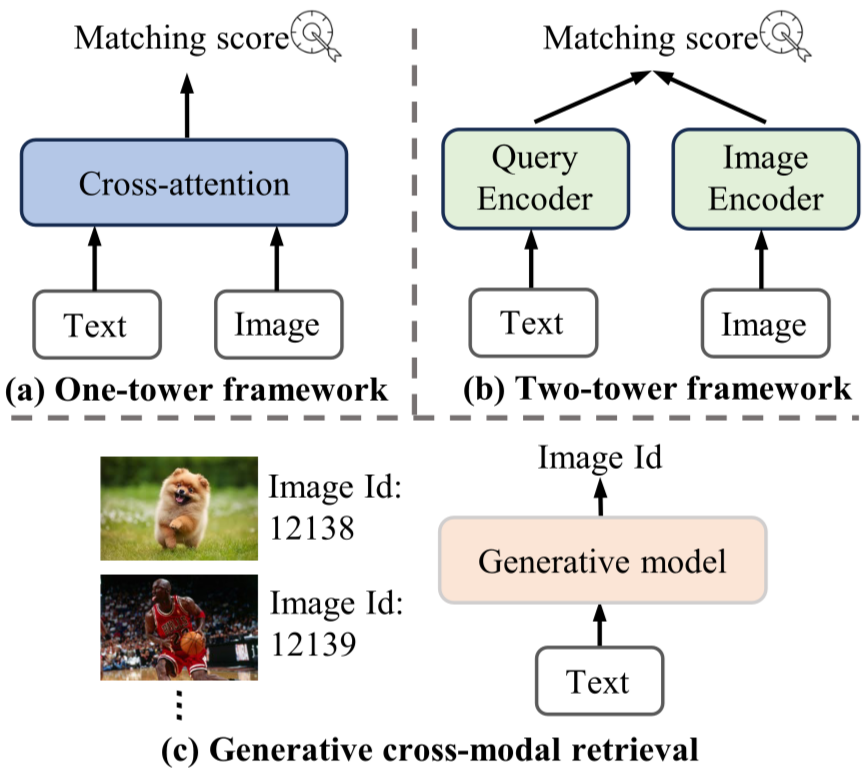
\includegraphics[width=0.86\textwidth,height=0.48\textheight,keepaspectratio]{retrieval.png}
\source{Retrieval formulation based on predicted scene-graph triplets; structured SGG motivation follows \href{https://openaccess.thecvf.com/content/CVPR2022/papers/Li_SGTR_End-to-End_Scene_Graph_Generation_With_Transformer_CVPR_2022_paper.pdf}{SGTR}.}
\end{talert}

% \centering
% \begin{tikzpicture}[node distance=1.5cm and 2.0cm, >=Stealth, every node/.style={font=\footnotesize}]
% \node[draw, rounded corners, fill=puregray, minimum width=2.7cm, minimum height=0.8cm] (q) {Text query $q$};
% \node[draw, rounded corners, fill=puregray, right=of q, minimum width=3.0cm, minimum height=0.8cm] (g) {Triplet index $\mathcal{G}(I)$};
% \node[draw, rounded corners, fill=pureorange!15, right=of g, minimum width=2.8cm, minimum height=0.8cm] (r) {Ranked images};
% \draw[->, thick] (q) -- node[above] {$\operatorname{sim}$} (g);
% \draw[->, thick] (g) -- node[above] {$\max$ score} (r);
% \end{tikzpicture}

\end{frame}


\begin{frame}[shrink=6]{Objectives and Scope}
\slidebody
\begin{talert}{Objectives}
\begin{enumerate}\slidesmall
  \item Build \textbf{PURE}: a compact directed-pair predicate model using dense visual evidence.
  \item Evaluate predicate ranking with both aggregate recall and mean recall: R@K and mR@K.
  \item Build \textbf{CORE}: a controlled diagnostic benchmark for relation sensitivity and retrieval stress tests.
  \item Demonstrate retrieval as a direct application of predicted relation triplets.
\end{enumerate}
\end{talert}

\begin{talert}{In-scope work}
\begin{enumerate}
    \item Vision-language relation scoring under the PredCls setting.
    \item Standardized Visual Genome dataset and custom CORE benchmark.
    \item Image retrieval demonstration via predicted relation triplets.
    \item Recent SGG architectures used as methodological context, not full reimplementation targets.
    \item Open-source components for computational feasibility and reproducibility.
\end{enumerate}
\end{talert}

\source{Scope follows the standard separation between PredCls, SGCls, and SGDet in \href{https://openaccess.thecvf.com/content_cvpr_2018/html/Zellers_Neural_Motifs_Scene_CVPR_2018_paper.html}{Neural Motifs}.}
\end{frame}

% =============================================================================
\section{Related Works}
\subsection{Positioning}

\begin{frame}{CLIP: Vision-Language Pretraining}
\slidebody
CLIP aligns image and text representations; PURE uses this shared space but adds directed relation states and predicate-specific scoring.

\vspace{0.25em}
\centering
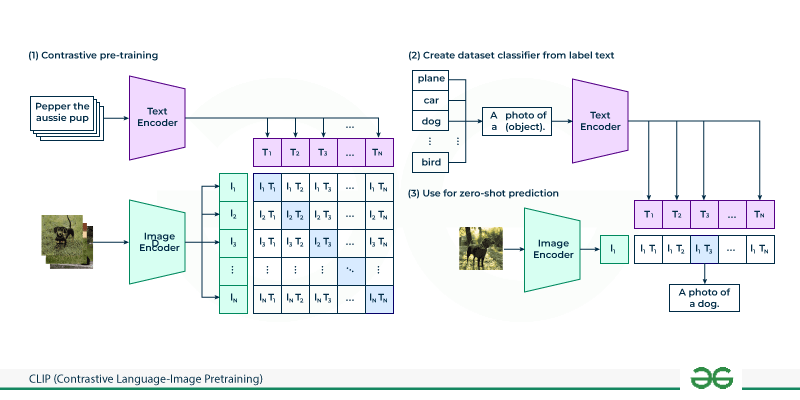
\includegraphics[width=0.92\textwidth,height=0.64\textheight,keepaspectratio]{clip.png}
\source{\href{https://arxiv.org/abs/2103.00020}{Radford et al., ``Learning Transferable Visual Models From Natural Language Supervision,'' ICML 2021}.}
\end{frame}

\begin{frame}{Neural Motifs: Context and Frequency Bias}
\slidebody
Neural Motifs defines a central VG-style SGG reference; it also shows why context and frequency priors must be separated from raw predicate scoring.

\vspace{0.25em}
\centering
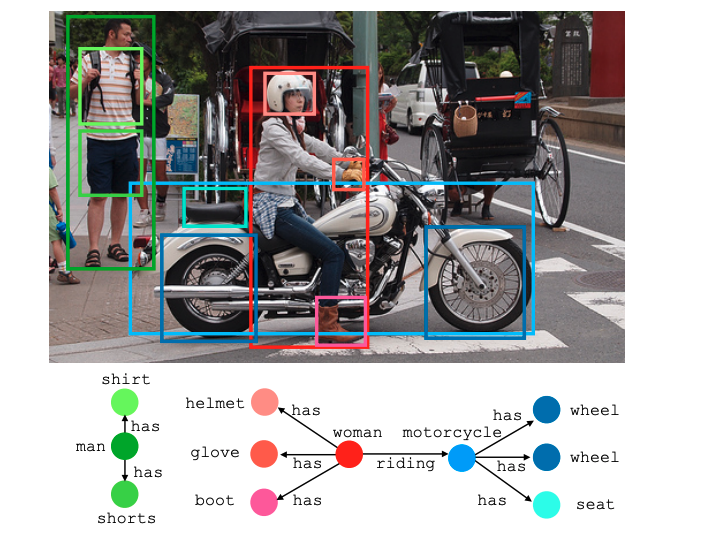
\includegraphics[width=0.92\textwidth,height=0.64\textheight,keepaspectratio]{neural_motifs.png}
\source{\href{https://openaccess.thecvf.com/content_cvpr_2018/html/Zellers_Neural_Motifs_Scene_CVPR_2018_paper.html}{Zellers et al., ``Neural Motifs: Scene Graph Parsing with Global Context,'' CVPR 2018}.}
\end{frame}

\begin{frame}{SGTR: Transformer-Based Relation Queries}
\slidebody
SGTR treats SGG as structured set prediction with relation queries; PURE keeps iterative relation refinement in a compact PredCls / GT-pair scorer.

\vspace{0.25em}
\centering
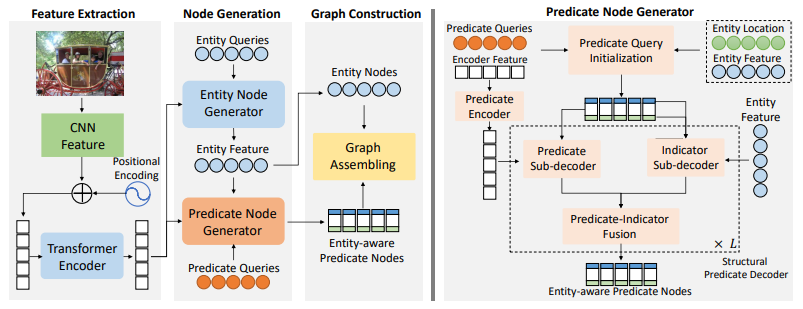
\includegraphics[width=0.92\textwidth,height=0.64\textheight,keepaspectratio]{sgtr.png}
\source{\href{https://openaccess.thecvf.com/content/CVPR2022/papers/Li_SGTR_End-to-End_Scene_Graph_Generation_With_Transformer_CVPR_2022_paper.pdf}{Li et al., ``SGTR: End-to-End Scene Graph Generation With Transformer,'' CVPR 2022}.}
\end{frame}


\begin{frame}{Other Works I: Debiasing Long-Tail Predicates}
\slidebody
\begin{talert}{Why SGG needs debiasing}
Visual Genome predicates are highly imbalanced: common relations such as ``on'', ``has'', or ``wearing'' dominate training, while rare but informative predicates receive fewer examples.
\begin{itemize}\footnotesize
  \item \textbf{TDE} separates visual evidence from dataset frequency bias at inference time.
  \item \textbf{CFA} creates compositional feature variants to strengthen rare predicate learning.
  \item \textbf{SBG} estimates sample-level bias, so hard or unusual samples receive different correction.
\end{itemize}
\end{talert}

\begin{talert}{Implication for PURE}
PURE reports both raw and calibrated scores: raw scores show learned visual relation evidence, while calibrated scores show the deployable ranking after frequency correction.
\end{talert}

\source{Sources: \href{https://openaccess.thecvf.com/content_cvpr_2020/html/Tang_Unbiased_Scene_Graph_Generation_From_Biased_Training_CVPR_2020_paper.html}{TDE}, \href{https://openaccess.thecvf.com/content/ICCV2023/html/Li_Compositional_Feature_Augmentation_for_Unbiased_Scene_Graph_Generation_ICCV_2023_paper.html}{CFA}, \href{https://eccv.ecva.net/virtual/2024/poster/2253}{SBG}.}
\end{frame}

\begin{frame}{Other Works II: Query-Based \& Open-Vocab SGG}
\slidebody
\begin{talert}{Structured relation prediction}
Transformer-based SGG models such as SGTR and RelTR move away from classifying independent object pairs only. They use relation queries to predict structured subject--predicate--object outputs.
\begin{itemize}\footnotesize
  \item This improves end-to-end graph generation, but makes training sensitive to assignment and sparse relation annotations.
  \item Recent Hydra-style SGG methods address this by giving one ground-truth relation multiple positive query matches.
\end{itemize}
\end{talert}

\begin{talert}{Open-vocabulary direction}
VLM-based SGG uses CLIP/LLM text spaces to score predicates beyond a fixed VG150 vocabulary. This motivates PURE's text-alignment head and the CORE diagnostic benchmark.
\end{talert}

\source{Sources: \href{https://openaccess.thecvf.com/content/CVPR2022/papers/Li_SGTR_End-to-End_Scene_Graph_Generation_With_Transformer_CVPR_2022_paper.pdf}{SGTR}, \href{https://arxiv.org/abs/2201.11460}{RelTR}, \href{https://arxiv.org/abs/2409.10262}{Hydra-SGG}, and \href{https://arxiv.org/abs/2404.00906}{open-vocabulary SGG/VLM literature}.}
\end{frame}
% =============================================================================
\section{Proposed Method}
\subsection{PURE Architecture}


\begin{frame}{PURE Overview}
\slidebody
PURE is a \textbf{relation scorer}: given object boxes and labels, it ranks possible predicates for every directed object pair.
\vspace{0.32em}

\centering
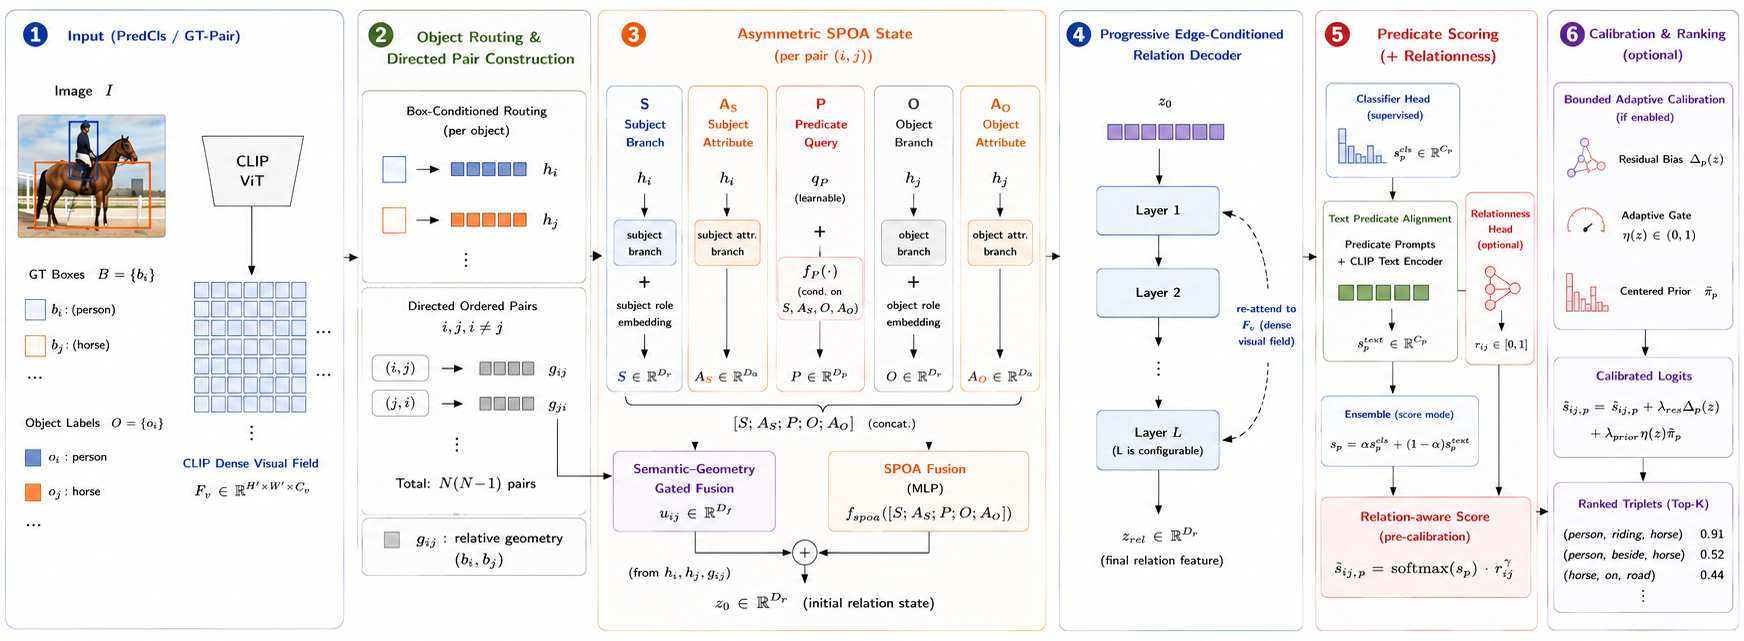
\includegraphics[width=\textwidth,height=0.74\textheight,keepaspectratio]{pipeline_diagram.png}

\source{PURE architecture from project implementation and assets; CLIP backbone context follows \href{https://arxiv.org/abs/2103.00020}{CLIP}.}
\end{frame}


\subsection{Dense Evidence and Pair Fusion}

\begin{frame}[shrink=9]{From Image to Object Evidence}
\slidebody
For each detected/ground-truth box, PURE gathers visual evidence from dense CLIP features instead of relying only on a cropped ROI.
\vspace{0.18em}

\centering
\makebox[\textwidth][c]{%
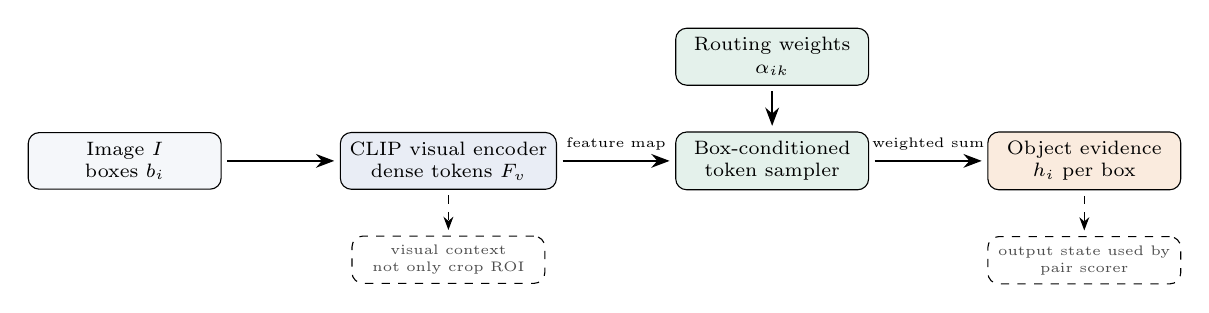
\begin{tikzpicture}[
  >=Stealth,
  shorten >=2pt,
  shorten <=2pt,
  font=\scriptsize,
  node distance=0.72cm and 1.50cm,
  mainbox/.style={draw, rounded corners, minimum width=2.45cm, minimum height=0.68cm, align=center},
  data/.style={mainbox, fill=puregray},
  vision/.style={mainbox, fill=pureblue!10},
  op/.style={mainbox, fill=puregreen!12},
  outputnode/.style={mainbox, fill=pureorange!15},
  note/.style={draw, dashed, rounded corners, fill=white, text=black!70, minimum width=2.45cm, minimum height=0.58cm, align=center, font=\tiny}
]
\node[data] (img) {Image $I$\\boxes $b_i$};
\node[vision, right=of img] (clip) {CLIP visual encoder\\dense tokens $F_v$};
\node[op, right=of clip] (sample) {Box-conditioned\\token sampler};
\node[op, above=0.58cm of sample] (attn) {Routing weights\\$\alpha_{ik}$};
\node[outputnode, right=of sample] (obj) {Object evidence\\$h_i$ per box};
\node[note, below=0.58cm of clip] (n1) {visual context\\not only crop ROI};
\node[note, below=0.58cm of obj] (n2) {output state used by\\pair scorer};
\draw[->, thick] (img) -- (clip);
\draw[->, thick] (clip) -- node[above, font=\tiny] {feature map} (sample);
\draw[->, thick] (sample) -- node[above, font=\tiny] {weighted sum} (obj);
\draw[->, thick] (attn) -- (sample);
\draw[->, dashed] (clip) -- (n1);
\draw[->, dashed] (obj) -- (n2);
\end{tikzpicture}
}

\vspace{0.18em}
\begin{talert}{Object-routing equation}
\[
h_i = \sum_{k=1}^{K} \alpha_{ik} F_v(p_{ik}), \qquad \sum_{k=1}^{K}\alpha_{ik}=1.
\]
{\footnotesize $h_i$ is box-level evidence; $F_v(p_{ik})$ is a dense CLIP token; $\alpha_{ik}$ is its learned importance.}
\end{talert}

\source{Project architecture diagram and implementation component: \href{https://arxiv.org/abs/2103.00020}{CLIP}-based \texttt{DeformableObjectRouter}.}
\end{frame}

\begin{frame}[shrink=14]{Directed Pair Fusion}
\slidebody
{\slidesmall Direction matters: ``person riding horse'' is not ``horse riding person'', so PURE builds a directed state for each ordered pair.}

\vspace{0.06em}
\centering
\makebox[\textwidth][c]{%
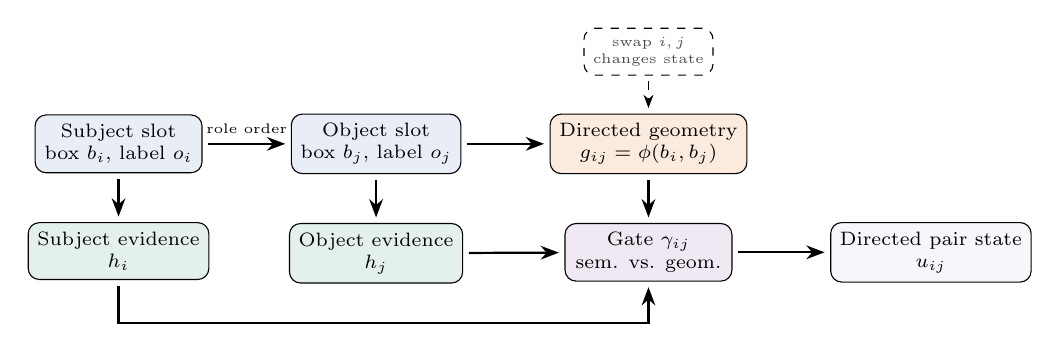
\begin{tikzpicture}[
  >=Stealth,
  shorten >=2pt,
  shorten <=2pt,
  font=\scriptsize,
  node distance=0.62cm and 1.12cm,
  pairbox/.style={draw, rounded corners, minimum width=2.12cm, minimum height=0.60cm, align=center},
  objnode/.style={pairbox, fill=pureblue!10},
  feat/.style={pairbox, fill=puregreen!12},
  geom/.style={pairbox, fill=pureorange!15},
  fuse/.style={pairbox, fill=purepurple!12},
  outputnode/.style={pairbox, fill=puregray},
  role/.style={draw, dashed, rounded corners, fill=white, text=black!70, align=center, font=\tiny}
]
\node[objnode] (sbox) {Subject slot\\box $b_i$, label $o_i$};
\node[objnode, right=of sbox] (obox) {Object slot\\box $b_j$, label $o_j$};
\node[feat, below=of sbox] (sfeat) {Subject evidence\\$h_i$};
\node[feat, below=of obox] (ofeat) {Object evidence\\$h_j$};
\node[geom, right=of obox] (gfeat) {Directed geometry\\$g_{ij}=\phi(b_i,b_j)$};
\node[fuse, below=of gfeat] (gate) {Gate $\gamma_{ij}$\\sem. vs. geom.};
\node[outputnode, right=1.24cm of gate] (pair) {Directed pair state\\$u_{ij}$};
\node[role, above=0.48cm of gfeat] (role) {swap $i,j$\\changes state};
\draw[->, thick] (sbox) -- (sfeat);
\draw[->, thick] (obox) -- (ofeat);
\draw[->, thick] (sbox.east) -- node[above, font=\tiny] {role order} (obox.west);
\draw[->, thick] (obox) -- (gfeat);
\draw[->, thick] (sfeat.south) |- ([yshift=-0.52cm]gate.south) -- (gate.south);
\draw[->, thick] (ofeat) -- (gate);
\draw[->, thick] (gfeat) -- (gate);
\draw[->, thick] (gate) -- (pair);
\draw[->, dashed] (role) -- (gfeat);
\end{tikzpicture}
}

\vspace{0.02em}
\begin{talert}{Semantic--geometry fusion}
\[
g_{ij}= \phi(b_i,b_j), \qquad
u_{ij}= \gamma_{ij}\, \mathrm{norm}(h_i+h_j)+(1-\gamma_{ij})\, \mathrm{norm}(g_{ij}).
\]
{\footnotesize $g_{ij}$ is directed geometry; $u_{ij}$ is pair evidence; $\gamma_{ij}$ balances semantics and layout.}
\end{talert}

\source{Project architecture diagram and implementation components; directed relation modeling follows \href{https://link.springer.com/article/10.1007/s11263-016-0981-7}{Visual Genome}.}
\end{frame}

\begin{frame}[shrink=21]{PURE: Asymmetric SPOA State}
\slidebody
SPOA stores relation evidence as \textbf{Subject}, subject \textbf{Attribute}, \textbf{Predicate}, \textbf{Object}, and object \textbf{Attribute}. Attributes help distinguish entities such as ``man in red shirt'' versus ``man in black jacket''.

\centering
\makebox[\textwidth][c]{%
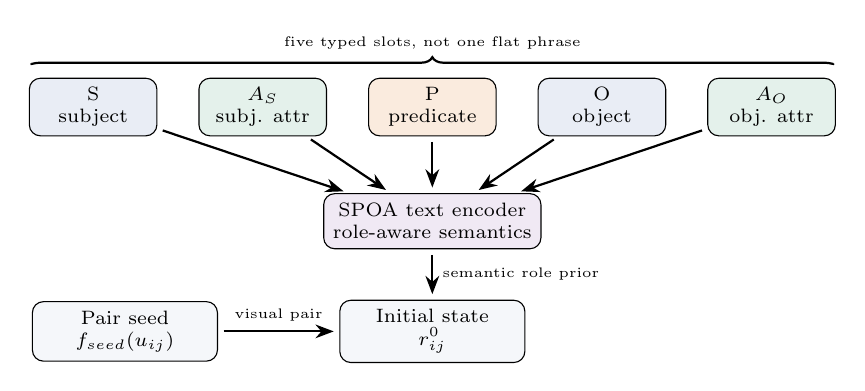
\begin{tikzpicture}[
  >=Stealth,
  shorten >=2pt,
  shorten <=2pt,
  font=\scriptsize,
  node distance=0.58cm and 0.52cm,
  slotbox/.style={draw, rounded corners, minimum width=1.62cm, minimum height=0.64cm, align=center},
  role/.style={slotbox, fill=pureblue!10},
  attr/.style={slotbox, fill=puregreen!12},
  pred/.style={slotbox, fill=pureorange!15},
  map/.style={draw, rounded corners, fill=purepurple!12, minimum width=2.35cm, minimum height=0.70cm, align=center},
  state/.style={draw, rounded corners, fill=puregray, minimum width=2.35cm, minimum height=0.70cm, align=center}
]
\node[role] (s) {S\\subject};
\node[attr, right=of s] (as) {$A_S$\\subj. attr};
\node[pred, right=of as] (p) {P\\predicate};
\node[role, right=of p] (o) {O\\object};
\node[attr, right=of o] (ao) {$A_O$\\obj. attr};
\node[map, below=0.72cm of p] (spoa) {SPOA text encoder\\role-aware semantics};
\node[state, below=0.64cm of spoa] (r0) {Initial state\\$r^0_{ij}$};
\node[state, left=1.54cm of r0] (pair) {Pair seed\\$f_{seed}(u_{ij})$};
\draw[decorate, decoration={brace, amplitude=4pt}, thick] ([yshift=0.12cm]s.north west) -- ([yshift=0.12cm]ao.north east) node[midway, yshift=0.32cm, font=\tiny] {five typed slots, not one flat phrase};
\draw[->, thick] (s) -- (spoa);
\draw[->, thick] (as) -- (spoa);
\draw[->, thick] (p) -- (spoa);
\draw[->, thick] (o) -- (spoa);
\draw[->, thick] (ao) -- (spoa);
\draw[->, thick] (pair) -- node[above, font=\tiny] {visual pair} (r0);
\draw[->, thick] (spoa) -- node[right, font=\tiny] {semantic role prior} (r0);
\end{tikzpicture}
}

\vspace{0.18em}
\begin{talert}{SPOA initialization}
\[
r^0_{ij}= f_{seed}(u_{ij}) + f_{spoa}([S;A_S;P;O;A_O]).
\]
{\footnotesize $r^0_{ij}$ is the initial state. The first term uses directed pair evidence; the second term injects role-aware SPOA semantics.}
\end{talert}

\source{SPOA state from current PURE implementation; relation directionality follows \href{https://link.springer.com/article/10.1007/s11263-016-0981-7}{Visual Genome}.}
\end{frame}

\subsection{SPOA Decoder and Scoring}

\begin{frame}[shrink=8]{PURE: Progressive Decoder}
\slidebody
The initial relation state is refined for several steps. At each step, it can re-attend to subject evidence, object evidence, dense visual context, and geometry.
\vspace{0.18em}

\centering
\makebox[\textwidth][c]{%
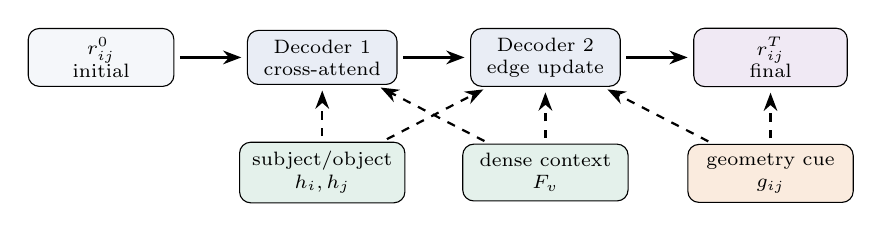
\begin{tikzpicture}[
  >=Stealth,
  shorten >=2pt,
  shorten <=2pt,
  font=\scriptsize,
  node distance=0.68cm and 0.92cm,
  state/.style={draw, rounded corners, fill=puregray, minimum width=1.85cm, minimum height=0.62cm, align=center},
  block/.style={draw, rounded corners, fill=pureblue!10, minimum width=1.90cm, minimum height=0.62cm, align=center},
  ctx/.style={draw, rounded corners, fill=puregreen!12, minimum width=2.10cm, minimum height=0.58cm, align=center},
  geom/.style={draw, rounded corners, fill=pureorange!15, minimum width=2.10cm, minimum height=0.58cm, align=center},
  outputnode/.style={draw, rounded corners, fill=purepurple!12, minimum width=1.95cm, minimum height=0.62cm, align=center}
]
\node[state] (r0) {$r^0_{ij}$\\initial};
\node[block, right=of r0] (d1) {Decoder 1\\cross-attend};
\node[block, right=of d1] (d2) {Decoder 2\\edge update};
\node[outputnode, right=of d2] (rt) {$r^T_{ij}$\\final};
\node[ctx, below=0.72cm of d1] (objctx) {subject/object\\$h_i,h_j$};
\node[ctx, below=0.72cm of d2] (dense) {dense context\\$F_v$};
\node[geom, below=0.72cm of rt] (geo) {geometry cue\\$g_{ij}$};
\draw[->, thick] (r0) -- (d1);
\draw[->, thick] (d1) -- (d2);
\draw[->, thick] (d2) -- (rt);
\draw[->, dashed, thick] (objctx) -- (d1);
\draw[->, dashed, thick] (objctx) -- (d2);
\draw[->, dashed, thick] (dense) -- (d1);
\draw[->, dashed, thick] (dense) -- (d2);
\draw[->, dashed, thick] (geo) -- (d2);
\draw[->, dashed, thick] (geo) -- (rt);
\end{tikzpicture}
}

\vspace{0.18em}
\begin{talert}{Refinement step}
\[
r^{t+1}_{ij}= \mathrm{LN}\left(r^t_{ij}+ \Delta_t(r^t_{ij}, h_i, h_j, g_{ij}, F_v)\right).
\]
{\footnotesize The update $\Delta_t$ is a small correction from subject/object features, geometry, and dense visual context; layer normalization keeps the state stable.}
\end{talert}

\source{Project architecture diagram and implementation component: \texttt{ProgressiveEdgeConditionedLayer}; iterative SGG context follows \href{https://openaccess.thecvf.com/content_cvpr_2017/html/Xu_Scene_Graph_Generation_CVPR_2017_paper.html}{IMP}.}
\end{frame}

\begin{frame}[shrink=8]{PURE: Predicate Scoring Heads}
\slidebody
PURE does not rely on one head only. It combines a closed-set classifier, a text-alignment score, and a relationness confidence.
\vspace{0.18em}

\centering
\makebox[\textwidth][c]{%
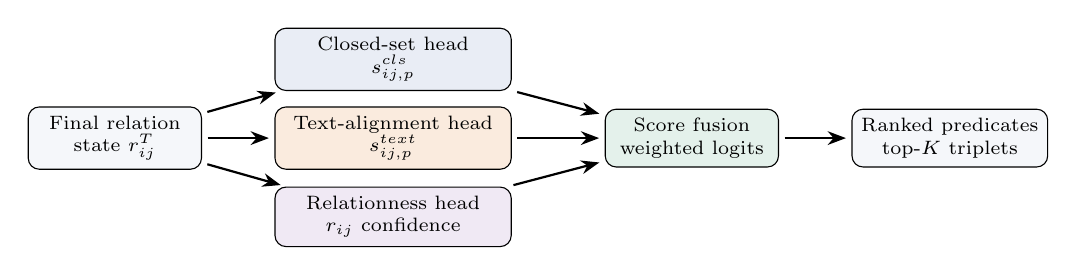
\begin{tikzpicture}[
  >=Stealth,
  shorten >=2pt,
  shorten <=2pt,
  font=\scriptsize,
  node distance=0.68cm and 0.92cm,
  scorebox/.style={draw, rounded corners, minimum width=2.20cm, minimum height=0.68cm, align=center},
  state/.style={scorebox, fill=puregray},
  head/.style={scorebox, minimum width=3cm, fill=pureblue!10},
  texthead/.style={scorebox, minimum width=3cm, fill=pureorange!15},
  relhead/.style={scorebox, minimum width=3cm, fill=purepurple!12},
  score/.style={scorebox, fill=puregreen!12},
  outputnode/.style={scorebox, fill=puregray}
]
\node[state] (r) {Final relation\\state $r^T_{ij}$};
\node[head, right=of r, yshift=1cm] (cls) {Closed-set head\\$s^{cls}_{ij,p}$};
\node[texthead, right=of r] (txt) {Text-alignment head\\$s^{text}_{ij,p}$};
\node[relhead, right=of r, yshift=-1cm] (rel) {Relationness head\\$r_{ij}$ confidence};
\node[score, right=1.18cm of txt] (score) {Score fusion\\weighted logits};
\node[outputnode, right=of score] (rank) {Ranked predicates\\top-$K$ triplets};
\draw[->, thick] (r) -- (cls);
\draw[->, thick] (r) -- (txt);
\draw[->, thick] (r) -- (rel);
\draw[->, thick] (cls) -- (score);
\draw[->, thick] (txt) -- (score);
\draw[->, thick] (rel) -- (score);
\draw[->, thick] (score) -- (rank);
\end{tikzpicture}
}

\vspace{0.18em}
\begin{talert}{Predicate score}
\[
s_{ij,p}= \alpha s^{cls}_{ij,p} + (1-\alpha)s^{text}_{ij,p} + \beta \log r_{ij}.
\]
{\footnotesize The classifier scores VG150 labels; the text head compares against predicate prompts; relationness $r_{ij}$ down-weights invalid object pairs.}
\end{talert}

\source{Project inference diagram and implementation components; text alignment context follows \href{https://arxiv.org/abs/2103.00020}{CLIP}.}
\end{frame}

\subsection{Training Objective and Calibration}

\begin{frame}{Training Objective}
\slidebody
\begin{talert}{Total loss}
\[
\mathcal{L}_{PURE}=
\lambda_{ce}\mathcal{L}_{PredCE\text{-}LA}
+\lambda_{spoa}\mathcal{L}_{CF\text{-}SPOA}
+\lambda_g\mathcal{L}_{Ground}.
\]
\begin{itemize}\footnotesize
  \item $\mathcal{L}_{PredCE\text{-}LA}$: predicate cross-entropy with logit adjustment for VG150 imbalance.
  \item $\mathcal{L}_{CF\text{-}SPOA}$: aligns visual relation states with correct text triplets and separates counterfactual negatives.
  \item $\mathcal{L}_{Ground}$: keeps relation evidence connected to dense visual tokens.
\end{itemize}
\end{talert}

\begin{talert}{Reading}
Classification gives accuracy, SPOA gives role sensitivity, and grounding reduces visually unsupported head-predicate shortcuts.
\end{talert}

\source{Losses from current PURE implementation; long-tail motivation follows \href{https://openaccess.thecvf.com/content_cvpr_2020/html/Tang_Unbiased_Scene_Graph_Generation_From_Biased_Training_CVPR_2020_paper.html}{TDE}.}
\end{frame}

\begin{frame}[shrink=11]{Calibration: Evaluation-Time Score Correction}
\slidebody
Calibration adjusts final predicate scores after training. It can boost or suppress predicates using learned residuals and frequency-prior information, but it does not change the trained model weights.
\vspace{0.18em}

\centering
\makebox[\textwidth][c]{%
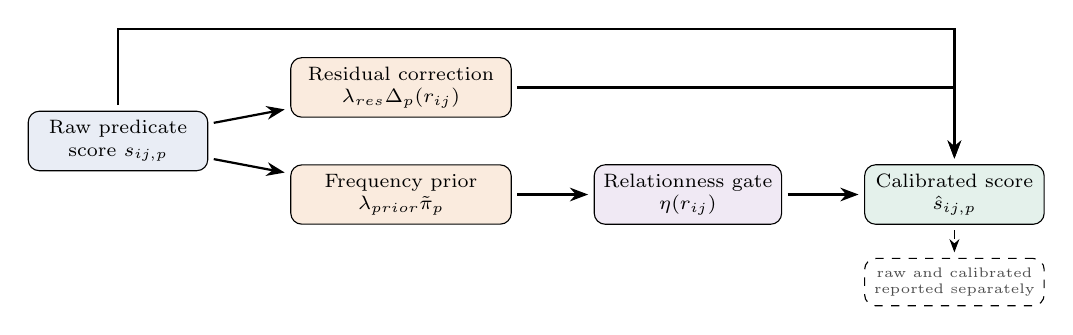
\begin{tikzpicture}[
  >=Stealth,
  shorten >=2pt,
  shorten <=2pt,
  font=\scriptsize,
  node distance=0.72cm and 1.04cm,
  calbox/.style={draw, rounded corners, minimum width=2.28cm, minimum height=0.64cm, align=center},
  raw/.style={calbox, fill=pureblue!10},
  corr/.style={calbox, minimum width=2.8cm, fill=pureorange!15},
  gate/.style={calbox, fill=purepurple!12},
  outputnode/.style={calbox, fill=puregreen!12},
  note/.style={draw, dashed, rounded corners, fill=white, text=black!70, minimum width=2.28cm, minimum height=0.56cm, align=center, font=\tiny}
]
\node[raw] (raw) {Raw predicate\\score $s_{ij,p}$};
\node[corr, right=of raw, yshift=0.68cm] (res) {Residual correction\\$\lambda_{res}\Delta_p(r_{ij})$};
\node[corr, right=of raw, yshift=-0.68cm] (prior) {Frequency prior\\$\lambda_{prior}\tilde{\pi}_p$};
\node[gate, right=of prior] (eta) {Relationness gate\\$\eta(r_{ij})$};
\node[outputnode, right=of eta] (hat) {Calibrated score\\$\hat{s}_{ij,p}$};
\node[note, below=0.42cm of hat] (note) {raw and calibrated\\reported separately};
\draw[->, thick] (raw.north) |- ([yshift=1.72cm]hat.north) -- (hat.north);
\draw[->, thick] (raw) -- (res);
\draw[->, thick] (raw) -- (prior);
\draw[->, thick] (res.east) -| (hat.north);
\draw[->, thick] (prior) -- (eta);
\draw[->, thick] (eta) -- (hat);
\draw[->, dashed] (hat) -- (note);
\end{tikzpicture}
}

\vspace{0.18em}
\begin{talert}{Calibrated score}
\[
\hat{s}_{ij,p}=s_{ij,p}+\lambda_{res}\Delta_p(r_{ij})+\lambda_{prior}\eta(r_{ij})\tilde{\pi}_p.
\]
{\footnotesize $s_{ij,p}$ is the raw score; residual and prior terms correct ranking bias at evaluation time. Raw and calibrated results are therefore reported separately.}
\end{talert}

\source{Project calibration plot and current PURE sweeps; long-tail calibration context follows \href{https://openaccess.thecvf.com/content_cvpr_2020/html/Tang_Unbiased_Scene_Graph_Generation_From_Biased_Training_CVPR_2020_paper.html}{TDE}.}
\end{frame}
\subsection{CORE Benchmark}

\begin{frame}[shrink=6]{CORE: Diagnostic Purpose}
\slidebody
CORE focuses on relation-sensitive retrieval cases generated from controlled counterfactual prompts.

\begin{talert}{What CORE tests}
\begin{itemize}
  \item Role sensitivity: whether subject and object are interpreted correctly.
  \item Attribute and spatial binding: whether modifiers and geometry attach to the right entity.
  \item Coverage: whether VG-compatible predicates are sufficient for diagnostic relations.
\end{itemize}

\begin{figure}
    \centering
    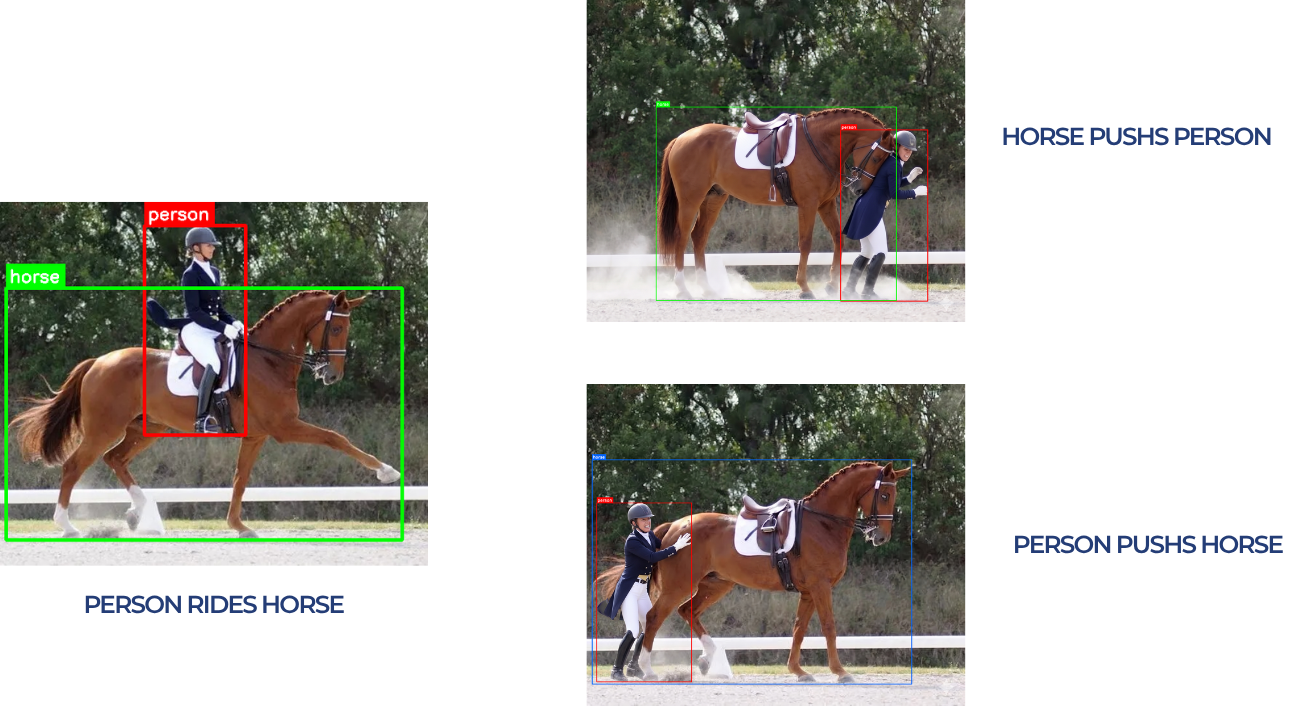
\includegraphics[width=0.42\linewidth]{pics/core_overview.png}
    \label{fig:core_overview}
\end{figure}

\end{talert}

\source{CORE is project-built; compositional evaluation motivation follows \href{https://arxiv.org/abs/2212.09645}{SugarCrepe}.}
\end{frame}

\begin{frame}{CORE Overview}
\slidebody
{\slidesmall CORE stands for Counterfactual Multi-label Relation Evaluation for Open-Vocabulary in the report assets; it is presented here as a controlled relation diagnostic resource.}

\vspace{0.15em}
\centering
\begin{minipage}{0.48\textwidth}
\centering
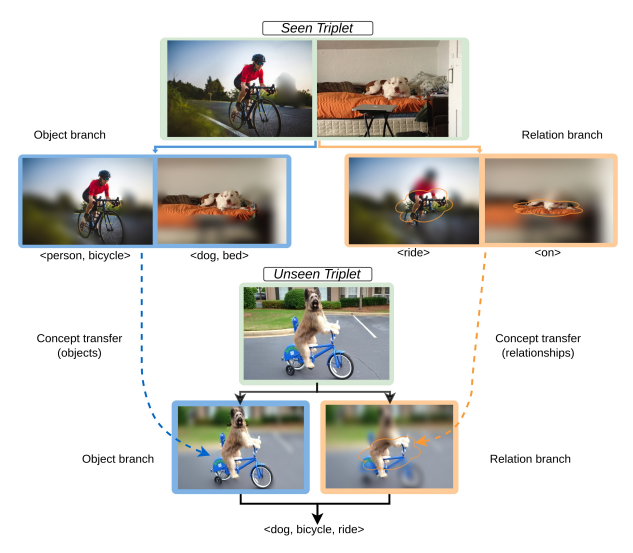
\includegraphics[width=\linewidth,height=0.80\textheight,keepaspectratio]{core_unseen.png}
\end{minipage}\hfill
\begin{minipage}{0.48\textwidth}
\centering
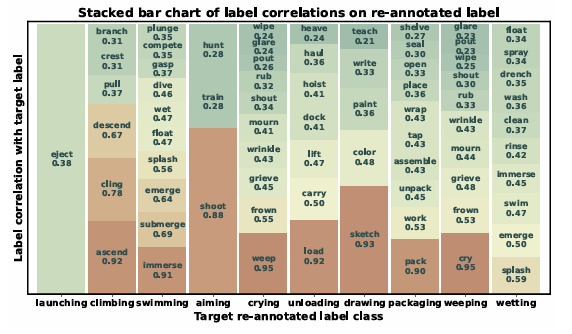
\includegraphics[width=\linewidth,height=0.63\textheight,keepaspectratio]{core_distribution.png}
\end{minipage}
\source{CORE overview and vocabulary-similarity distribution from project analysis; compositional evaluation motivation follows \href{https://arxiv.org/abs/2212.09645}{SugarCrepe}.}
\end{frame}

\begin{frame}{CORE Generation Pipeline}
\slidebody
{\slidesmall The generation pipeline combines prompt design, synthetic images, box extraction, and human/VLM audit before evaluation.}

\vspace{0.5em}
\centering
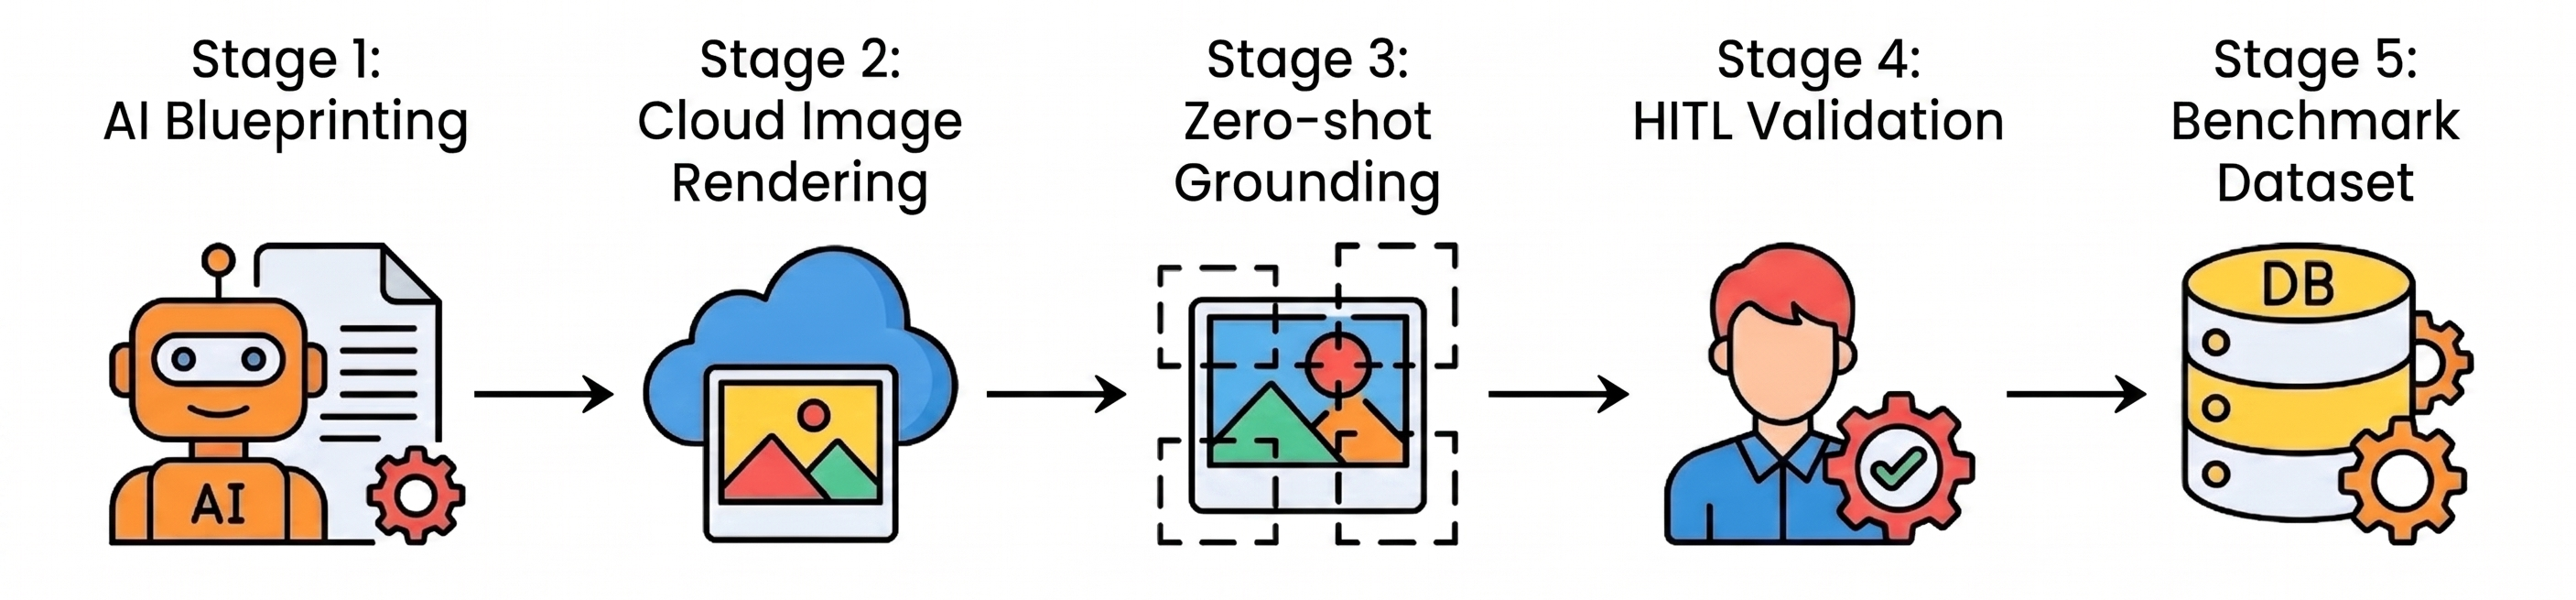
\includegraphics[width=\textwidth,height=0.64\textheight,keepaspectratio]{core_pipeline.png}
\source{Project CORE generation pipeline; open-set grounding context follows \href{https://arxiv.org/abs/2303.05499}{Grounding DINO}.}
\end{frame}

\begin{frame}{CORE Example: Action Role Reversal}
\slidebody
{\slidesmall This group probes who performs the action and who receives it.}

\vspace{0.15em}
\centering
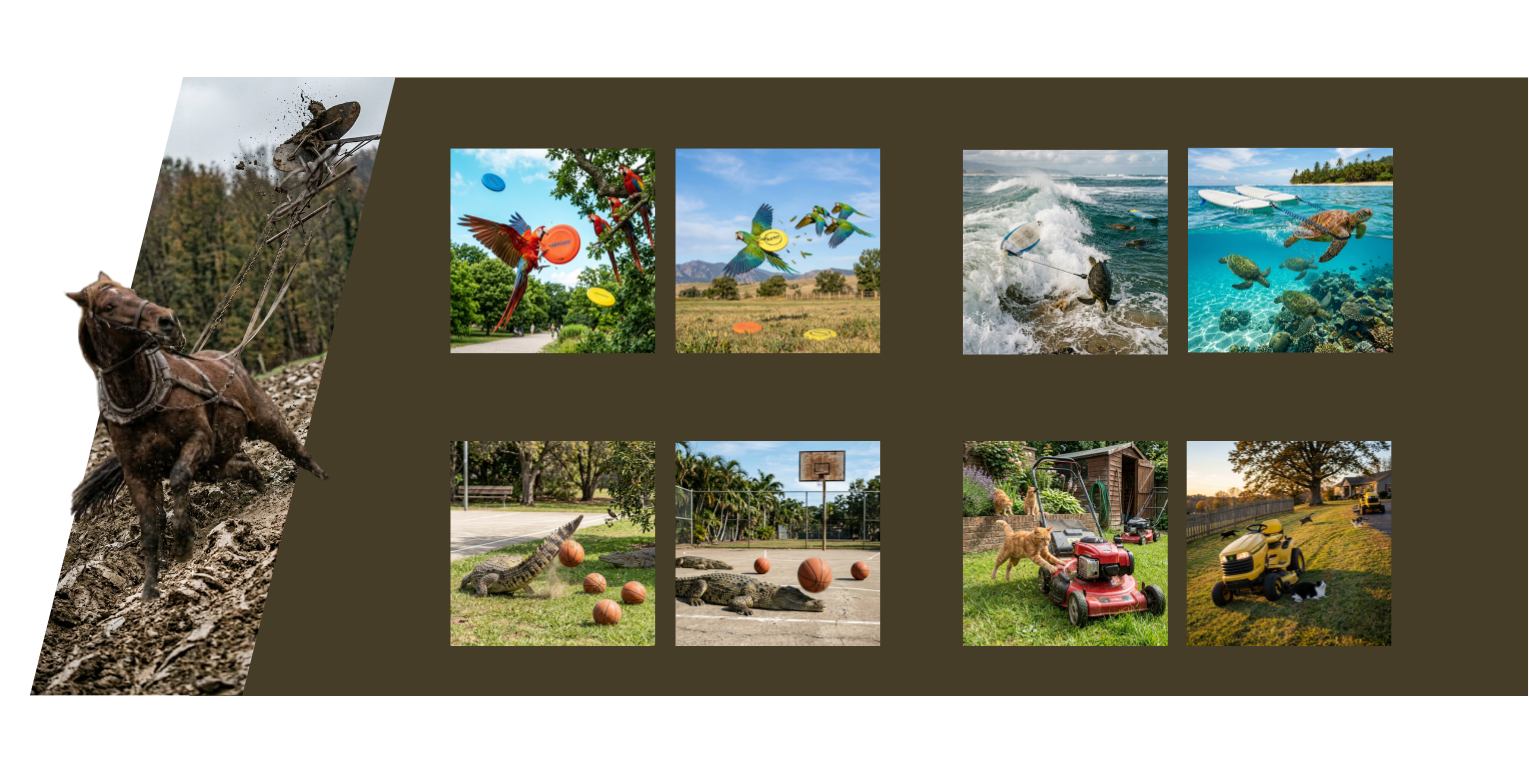
\includegraphics[width=\textwidth,height=0.80\textheight,keepaspectratio]{core_action_role.png}
\source{CORE diagnostic group from project benchmark; compositional evaluation context follows \href{https://arxiv.org/abs/2212.09645}{SugarCrepe}.}
\end{frame}

\begin{frame}{CORE Example: Attribute Binding}
\slidebody
{\slidesmall Attribute cases test whether modifiers attach to the intended entity.}

\vspace{0.15em}
\centering
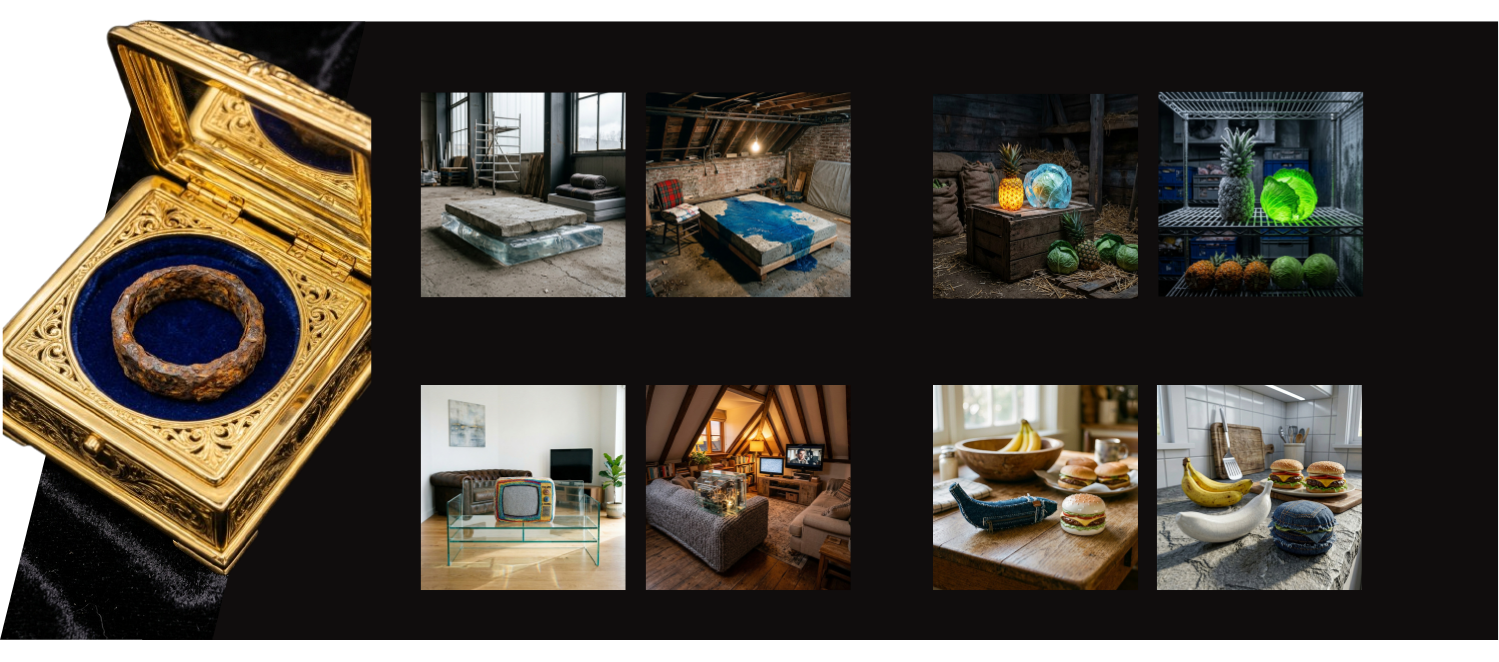
\includegraphics[width=\textwidth,height=0.72\textheight,keepaspectratio]{core_attribute_binding.png}
\source{CORE diagnostic group from project benchmark; compositional evaluation context follows \href{https://arxiv.org/abs/2212.09645}{SugarCrepe}.}
\end{frame}

\begin{frame}{CORE Example: Spatial and Containment}
\slidebody
{\slidesmall Spatial cases test support, containment, and relative layout beyond object co-occurrence.}

\vspace{0.15em}
\centering
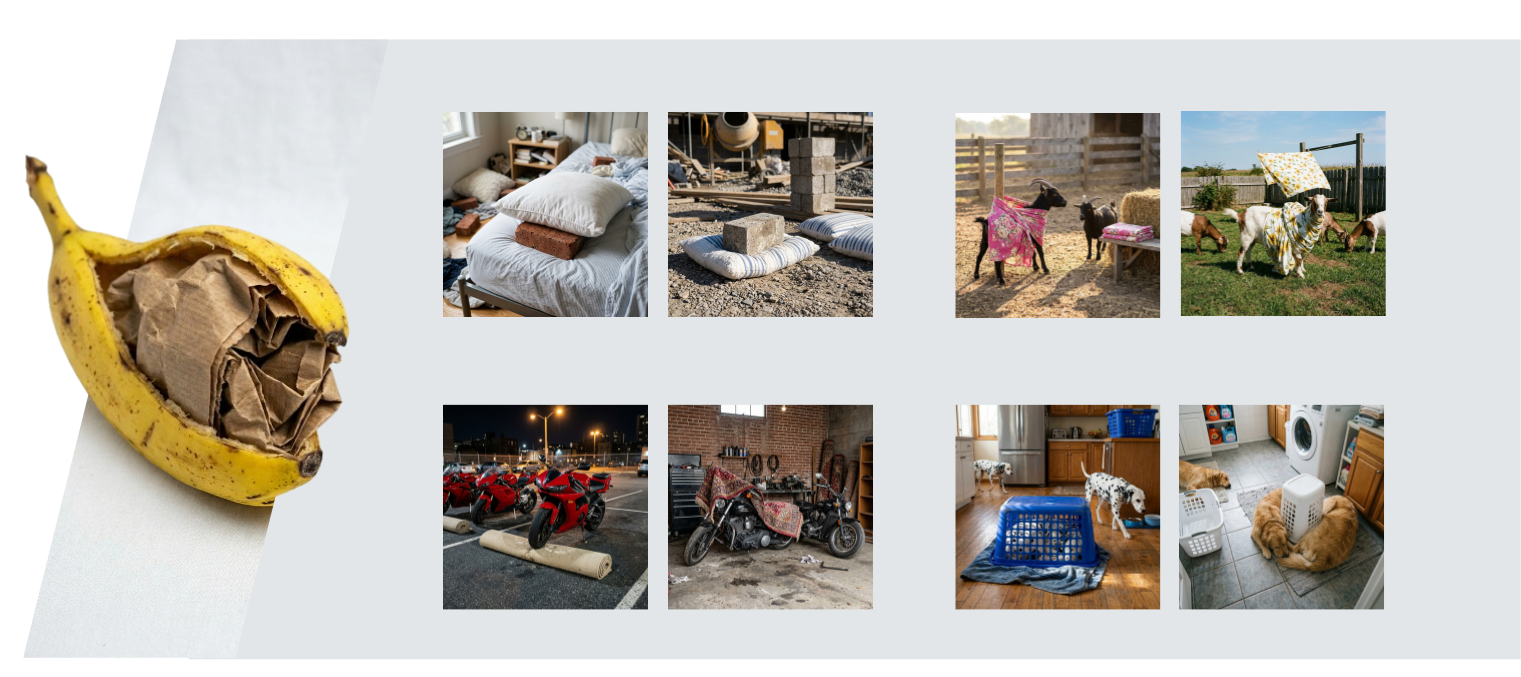
\includegraphics[width=\textwidth,height=0.72\textheight,keepaspectratio]{core_spatial_containment.png}
\source{CORE diagnostic group from project benchmark; compositional evaluation context follows \href{https://arxiv.org/abs/2212.09645}{SugarCrepe}.}
\end{frame}

\begin{frame}{CORE Example: Gaze and Attention}
\slidebody
{\slidesmall Gaze cases test whether attention direction is grounded in the subject-object pair.}

\vspace{0.15em}
\centering
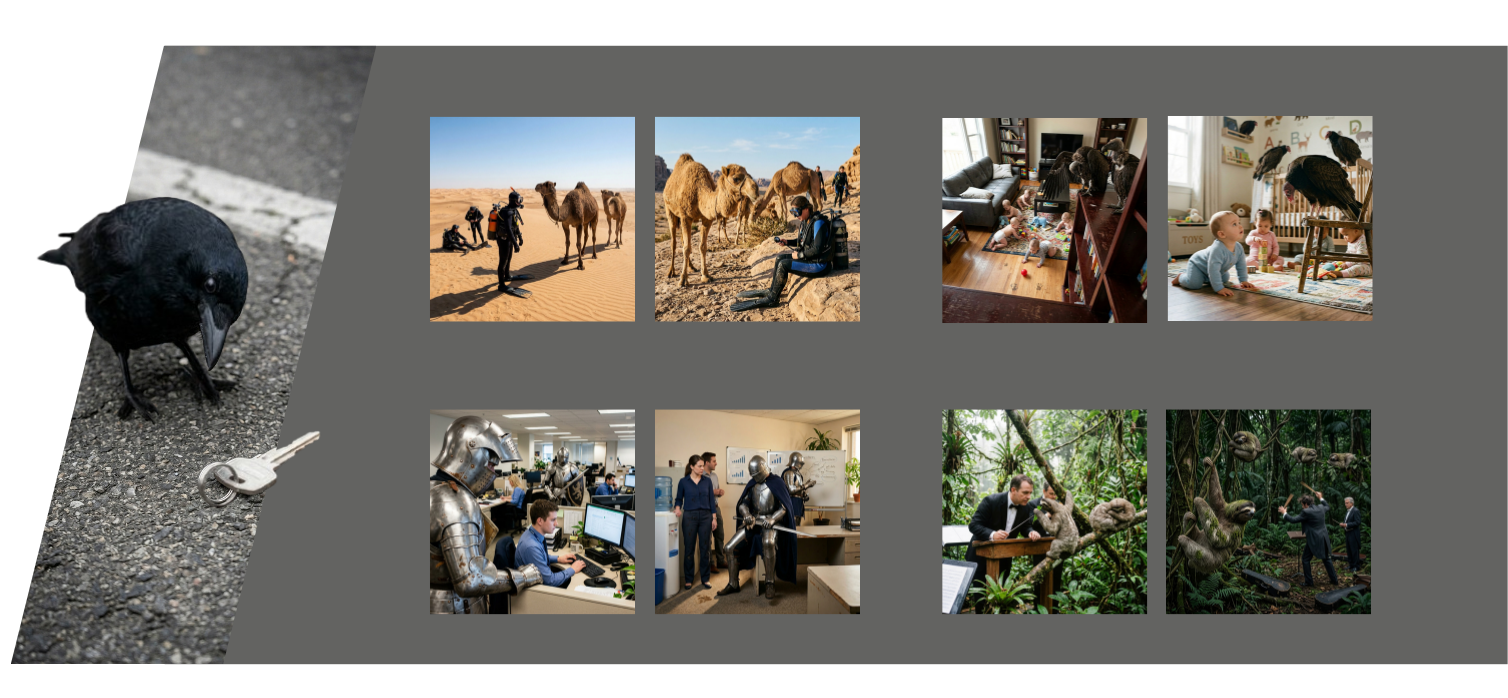
\includegraphics[width=\textwidth,height=0.72\textheight,keepaspectratio]{core_gaze_attention.png}
\source{CORE diagnostic group from project benchmark; compositional evaluation context follows \href{https://arxiv.org/abs/2212.09645}{SugarCrepe}.}
\end{frame}

\begin{frame}{CORE Example: Occlusion and Depth}
\slidebody
{\slidesmall Depth and occlusion cases reveal whether spatial evidence is used directionally.}

\vspace{0.15em}
\centering
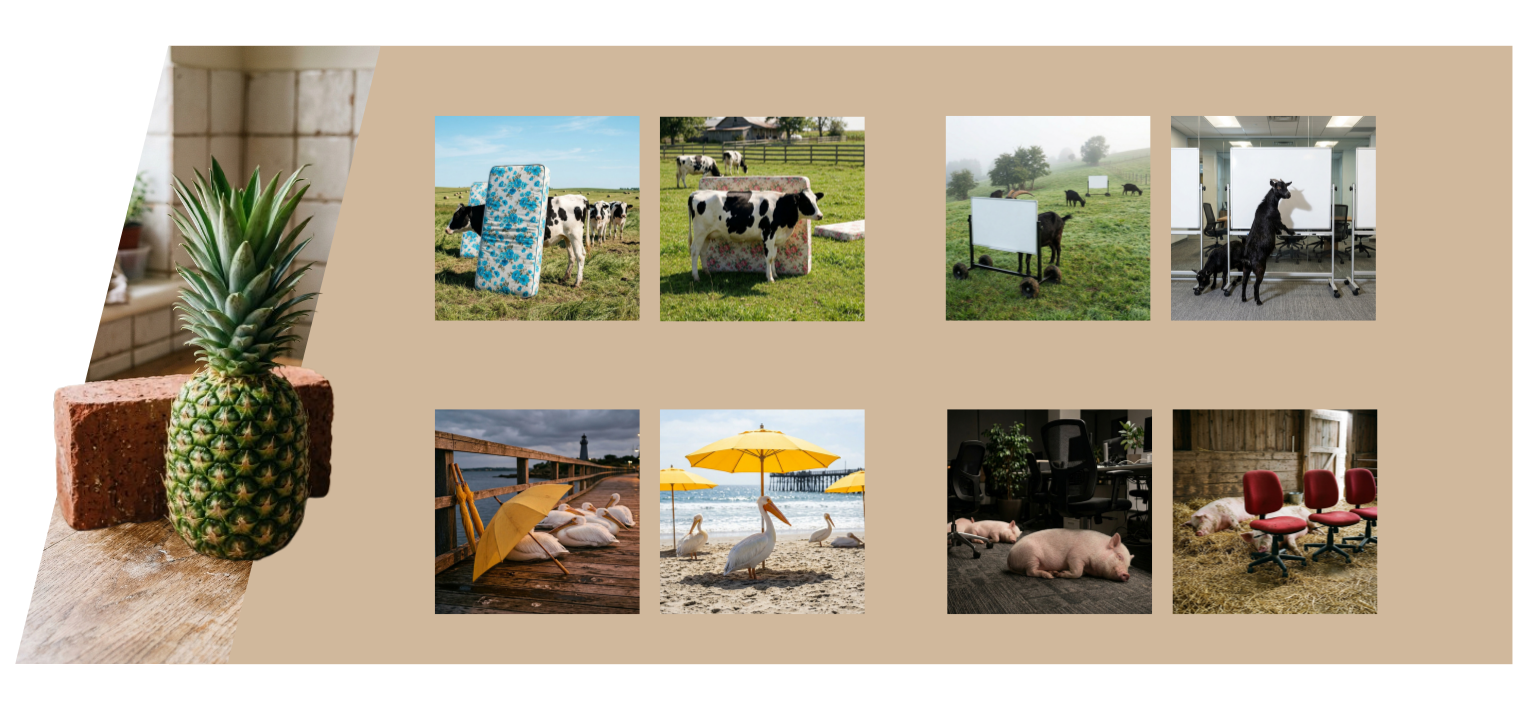
\includegraphics[width=\textwidth,height=0.72\textheight,keepaspectratio]{core_occlusion_depth.png}
\source{CORE diagnostic group from project benchmark; compositional evaluation context follows \href{https://arxiv.org/abs/2212.09645}{SugarCrepe}.}
\end{frame}

\begin{frame}{CORE Example: Extreme Compositional OOD}
\slidebody
{\slidesmall Extreme OOD cases test unusual object-relation compositions with limited VG-compatible coverage.}

\vspace{0.15em}
\centering
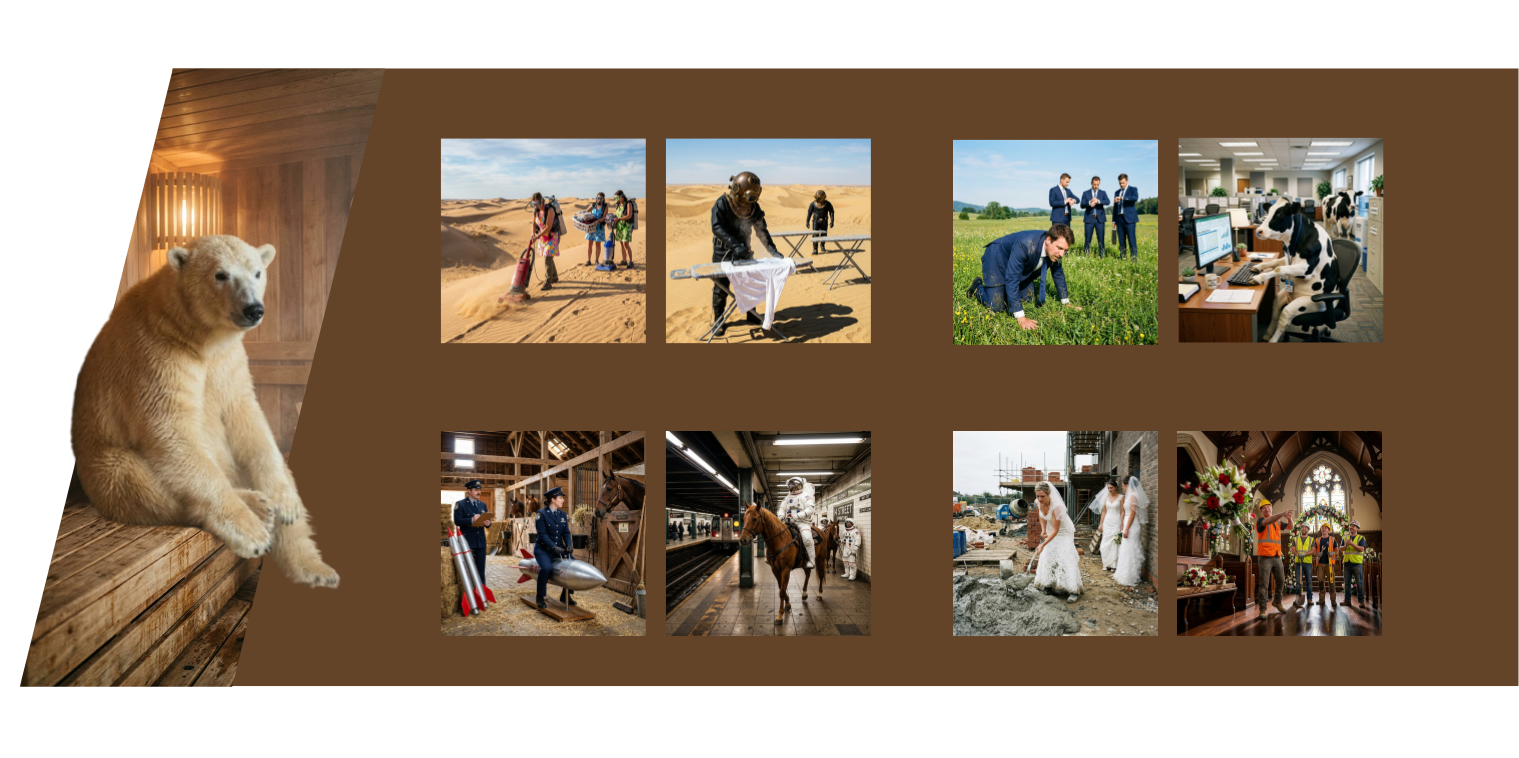
\includegraphics[width=\textwidth,height=0.72\textheight,keepaspectratio]{core_extreme_ood.png}
\source{CORE diagnostic group from project benchmark; compositional evaluation context follows \href{https://arxiv.org/abs/2212.09645}{SugarCrepe}.}
\end{frame}

% =============================================================================
\section{Experiments and Discussion}
\subsection{Datasets, Metrics, and Setup}


\begin{frame}[fragile,shrink=4]{VG150 Metadata}
VG150 is the main evaluation dataset. It is derived from Visual Genome and uses a fixed SGG vocabulary for protocol-compatible PredCls evaluation.

\vspace{1em}
\begin{columns}[T]

    % Cột đệm 1: Tạo khoảng trống bên trái để đẩy ảnh/bảng sang phải
    \begin{column}{0.04\textwidth}
    \end{column}

    % Cột 2: Ảnh và Bảng (Đã kéo lên trên và thu nhỏ)
    \begin{column}{0.36\textwidth}
        \vspace*{0pt}
        \vspace*{-1.2em} % Kéo toàn bộ ảnh và bảng lên trên
        \centering
        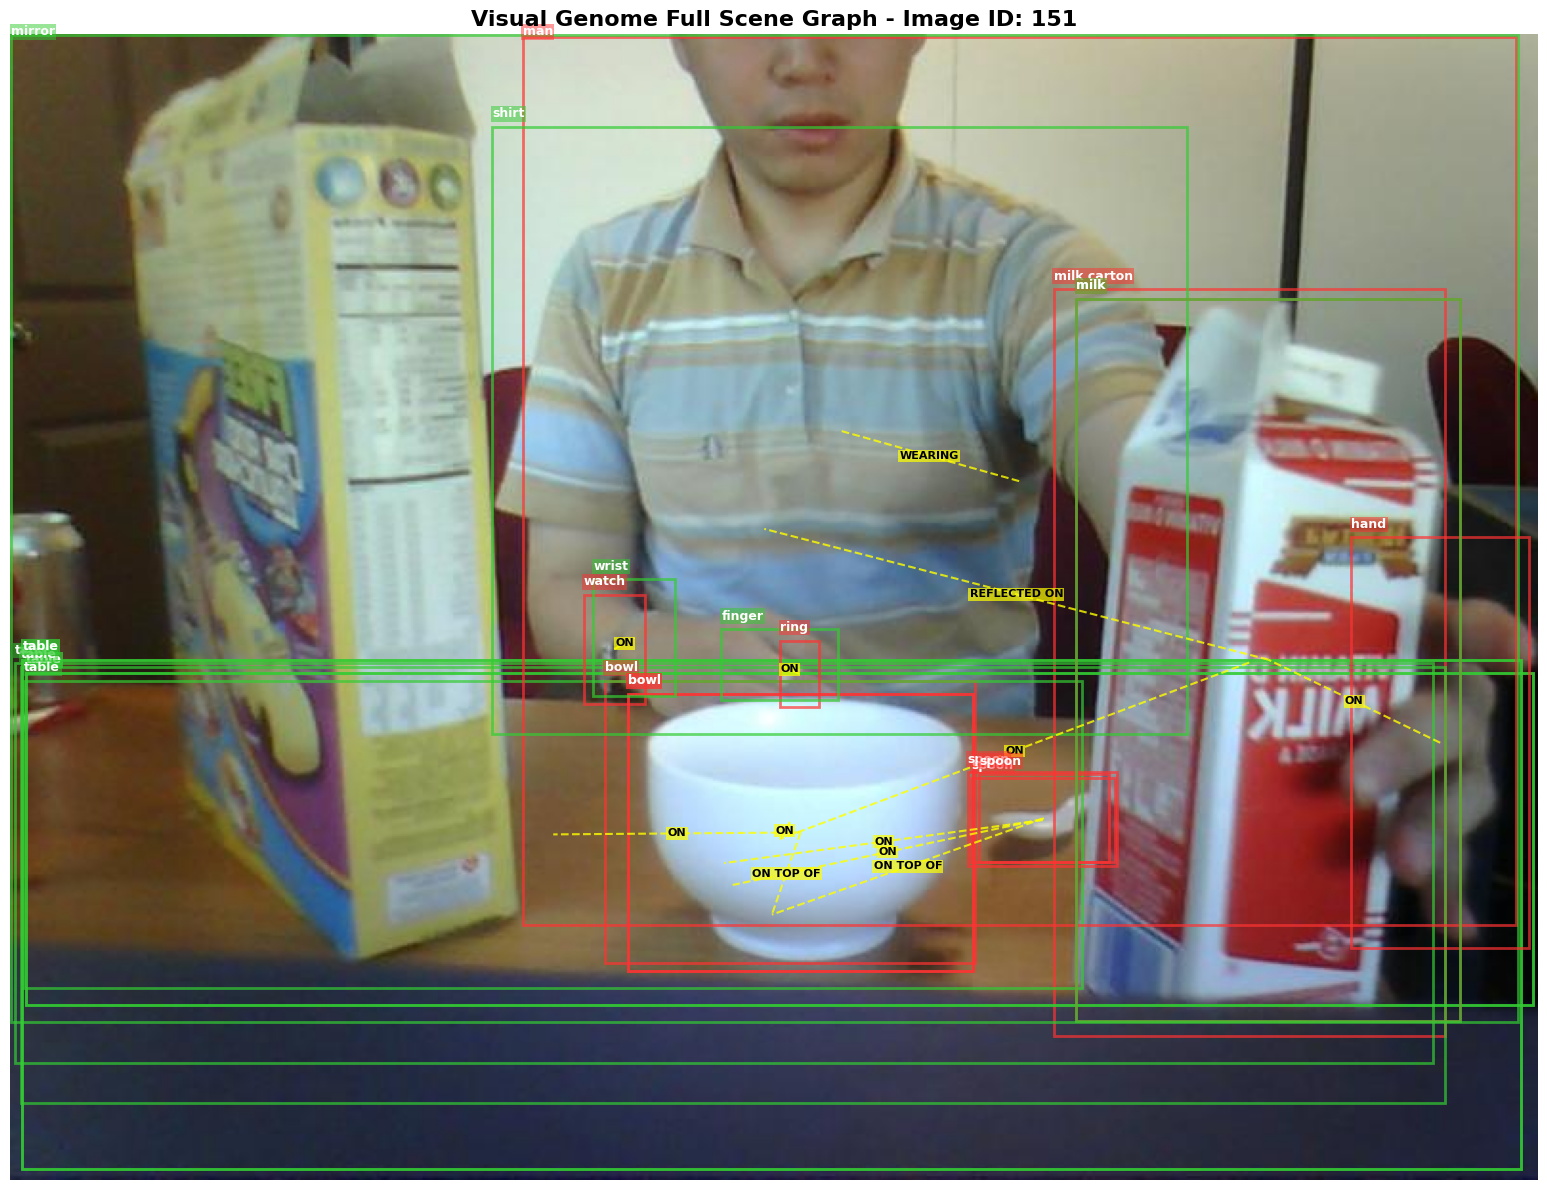
\includegraphics[width=\textwidth,keepaspectratio]{vg_sample.png}
        
        \vspace{0.5em} % Khoảng cách giữa ảnh và bảng
        
        % Thu nhỏ bảng gọn gàng
        \renewcommand{\arraystretch}{0.85} 
        \resizebox{0.95\textwidth}{!}{
            \begin{tabular}{lc}
            \toprule
            \textbf{Metric} & \textbf{Value} \\
            \midrule
            Total images & 108,077 \\
            Total regions & 5,408,689 \\
            Avg. regions per image & 50.04 ($\sigma = 9.25$) \\
            Avg. coverage & 548.61\% \\
            Vocabulary size & 94,244 \\
            Avg. description length & 5.0 words \\
            Word entropy & 5.8953 \\
            Bigram entropy & 9.4997 \\
            Sampled IoU & 0.0593 \\
            \bottomrule
            \end{tabular}
        }
    \end{column}

    % Cột đệm 2: Giữ khoảng cách giữa ảnh và JSON
    \begin{column}{0.02\textwidth}
    \end{column}

    % Cột 3: JSON và Source (Giữ nguyên cấu trúc)
    \begin{column}{0.56\textwidth}
        \vspace*{0pt}
        \vspace*{-1.8em} % Kéo Verbatim lên trên
        \fontsize{4.2pt}{5.0pt}\selectfont
\begin{verbatim}
{
  "image_metadata": {
    "width": 800, "height": 600, 
    "image_id": 151, "coco_id": null, "flickr_id": null,
    "url": "https://cs.stanford.edu/people/rak248/VG_100K_2/151.jpg"
  },
  "relationships": [
    {
      "relationship_id": 4256404, 
      "predicate": "ON", 
      "synsets": ["along.r.01"],
      "subject": {
        "name": "milk carton", 
        "object_id": 3792908, 
        "x": 546, 
        "y": 133, 
        "w": 205, 
        "h": 391, 
        "synsets": []
      },
      "object": {
        "name": "table", 
        "object_id": 3792910, 
        "x": 8, 
        "y": 334, 
        "w": 789, 
        "h": 174, 
        "synsets": ["table.n.02"]
      }
    },
    // 11 other relationships...
  ]
}
\end{verbatim}
        
        \vspace{-0.5em}
        
        \fontsize{4pt}{5pt}\selectfont
        \textit{Source: Dataset: \href{https://link.springer.com/article/10.1007/s11263-016-0981-7}{Visual Genome}; VG150 protocol: \href{https://openaccess.thecvf.com/content_cvpr_2018/html/Zellers_Neural_Motifs_Scene_CVPR_2018_paper.html}{Neural Motifs}.}
    \end{column}
    
\end{columns}
\end{frame}

\begin{frame}{VG150 Metadata}

\begin{talert}{Evaluation metadata}
\begin{itemize}
  \item Input annotations: object boxes $B$, object labels $O$, and relation triplets $(s_i,p_{ij},o_j)$.
  \item Main protocol: PredCls / GT-pair, isolating predicate ranking from object detection.
  \item Main concern: predicate frequencies are long-tailed, so R@K and mR@K must be read together.
\end{itemize}
\end{talert}

\slidebody
\begin{table}[htbp]
\centering
\footnotesize
\begin{tabular}{p{27mm} p{100mm}}
\toprule
\textbf{Item} & \textbf{Setting} \\
\midrule
Dataset source & Visual Genome, standardized as VG150 for SGG. \\
Input annotations & Ground-truth boxes $B$, object labels $O$, and relation triplets $(s_i,p_{ij},o_j)$. \\
Main protocol & PredCls / GT-pair: evaluate predicate ranking with objects fixed. \\
Main metrics & R@50 for aggregate recall and mR@50 for long-tail predicate balance. \\
Main readout & Raw classifier scores and calibrated scores are reported as separate operating points. \\
\bottomrule
\end{tabular}
\end{table}
\source{Report experimental setup; VG150 protocol follows \href{https://openaccess.thecvf.com/content_cvpr_2018/html/Zellers_Neural_Motifs_Scene_CVPR_2018_paper.html}{Neural Motifs}.}
\end{frame}

\subsection{Metrics}

\begin{frame}[shrink=5]{VG150 and Metrics}
\slidebody
VG150 is derived from Visual Genome and uses a restricted set of frequent object and predicate classes for SGG evaluation. Because predicates are long-tailed, one aggregate metric is not enough.

\begin{talert}{Recall at K}
\[
R@K=\frac{\#\{\text{ground-truth triplets recovered in top }K\}}{\#\{\text{ground-truth triplets}\}}.
\]
R@K measures aggregate ranking quality but can be dominated by frequent predicates.
\end{talert}

\begin{talert}{Mean Recall at K}
\[
mR@K=\frac{1}{|\mathcal{P}|}\sum_{p\in\mathcal{P}}R_p@K.
\]
Mean recall is the main long-tail diagnostic because each predicate contributes equally.
\end{talert}

\source{Visual Genome dataset: \href{https://link.springer.com/article/10.1007/s11263-016-0981-7}{Krishna et al., IJCV 2017}; protocol follows \href{https://openaccess.thecvf.com/content_cvpr_2018/html/Zellers_Neural_Motifs_Scene_CVPR_2018_paper.html}{Neural Motifs}.}
\end{frame}

\begin{frame}{Training Configuration}
\slidebody
The maintained run uses the current L4 script with dense CLIP features and relation-specific heads enabled.

\begin{table}[htbp]
\centering
\footnotesize
\begin{tabular}{p{30mm} p{88mm}}
\toprule
\textbf{Configuration} & \textbf{Setting} \\
\midrule
Hardware preset & NVIDIA L4 24GB, single GPU. \\
Precision & AMP bf16, channels-last layout, TF32 when available. \\
Optimization & 6 epochs, batch 12, accumulation 2, gradient checkpointing. \\
Routing budget & Input 448, max objects 32, max pairs 64, learned prune $K=64$. \\
Evaluation & PredCls / GT-pair with raw and calibrated score readouts. \\
\bottomrule
\end{tabular}
\end{table}
\source{Maintained script: \texttt{scripts/train\_l4\_phase34.sh}; CLIP adaptation context follows \href{https://arxiv.org/abs/2103.00020}{CLIP}.}
\end{frame}

\begin{frame}{Training Schedule and Presets}
\slidebody
\begin{table}[htbp]
\centering
\scriptsize
\begin{tabular}{p{23mm} p{27mm} p{75mm}}
\toprule
\textbf{Preset / step} & \textbf{Where used} & \textbf{Meaning} \\
\midrule
Warmup & Training & Keep CLIP stable while relation heads and SPOA alignment start learning. \\
Adapt-light & Training + calibration & Controlled adaptation for relation-sensitive features and fixed-prior sweeps. \\
Ultra-light & Raw baseline & Low-VRAM preset to test relation-head behavior with minimal adaptation. \\
Prior-only & Ablation & Measures how much improvement comes from statistical prior scoring. \\
Calibration sweep & Evaluation & Fixed-prior calibration strengths applied to logits at inference. \\
\bottomrule
\end{tabular}
\end{table}
\source{Report training-schedule and run-preset tables; calibration schedule context follows \href{https://openaccess.thecvf.com/content_cvpr_2020/html/Tang_Unbiased_Scene_Graph_Generation_From_Biased_Training_CVPR_2020_paper.html}{TDE}.}
\end{frame}


\subsection{Quantitative Results}

\begin{frame}{Main PredCls Results}
Calibration strongly improves aggregate R@50. Raw runs remain important because they reveal what the learned predicate scorer can do before score redistribution.

\slidebody
\begin{table}[htbp]
\centering
\tablesize
\begin{tabular}{p{30mm} c c p{45mm}}
\toprule
\textbf{Configuration} & \textbf{R@50} & \textbf{mR@50} & \textbf{Reading} \\
\midrule
\textbf{Adapt-light + fa45} & \textbf{67.20} & 22.74 & Best aggregate recall. \\
\textbf{Adapt-light + fa375} & 67.09 & \textbf{22.99} & Best calibrated mean recall. \\
Ultra-light raw e2 & 35.22 & 20.35 & Strong raw tail behavior. \\
Adapt-light raw e5 & 33.71 & 20.03 & Tail improves with later epoch. \\
Prior-only raw e5 & 33.50 & 19.50 & Prior baseline below Adapt-light. \\
\bottomrule
\end{tabular}
\end{table}

\source{Project VG150 PredCls logs; dataset/protocol: \href{https://link.springer.com/article/10.1007/s11263-016-0981-7}{Visual Genome}, \href{https://openaccess.thecvf.com/content_cvpr_2018/html/Zellers_Neural_Motifs_Scene_CVPR_2018_paper.html}{Neural Motifs}.}
\end{frame}


\begin{frame}{Training Loss Plot}
\slidebody
{\slidesmall Training curves support the later ablation reading: predicate classification, SPOA alignment, and grounding stabilize together during optimization.}

\vspace{0.15em}
\centering
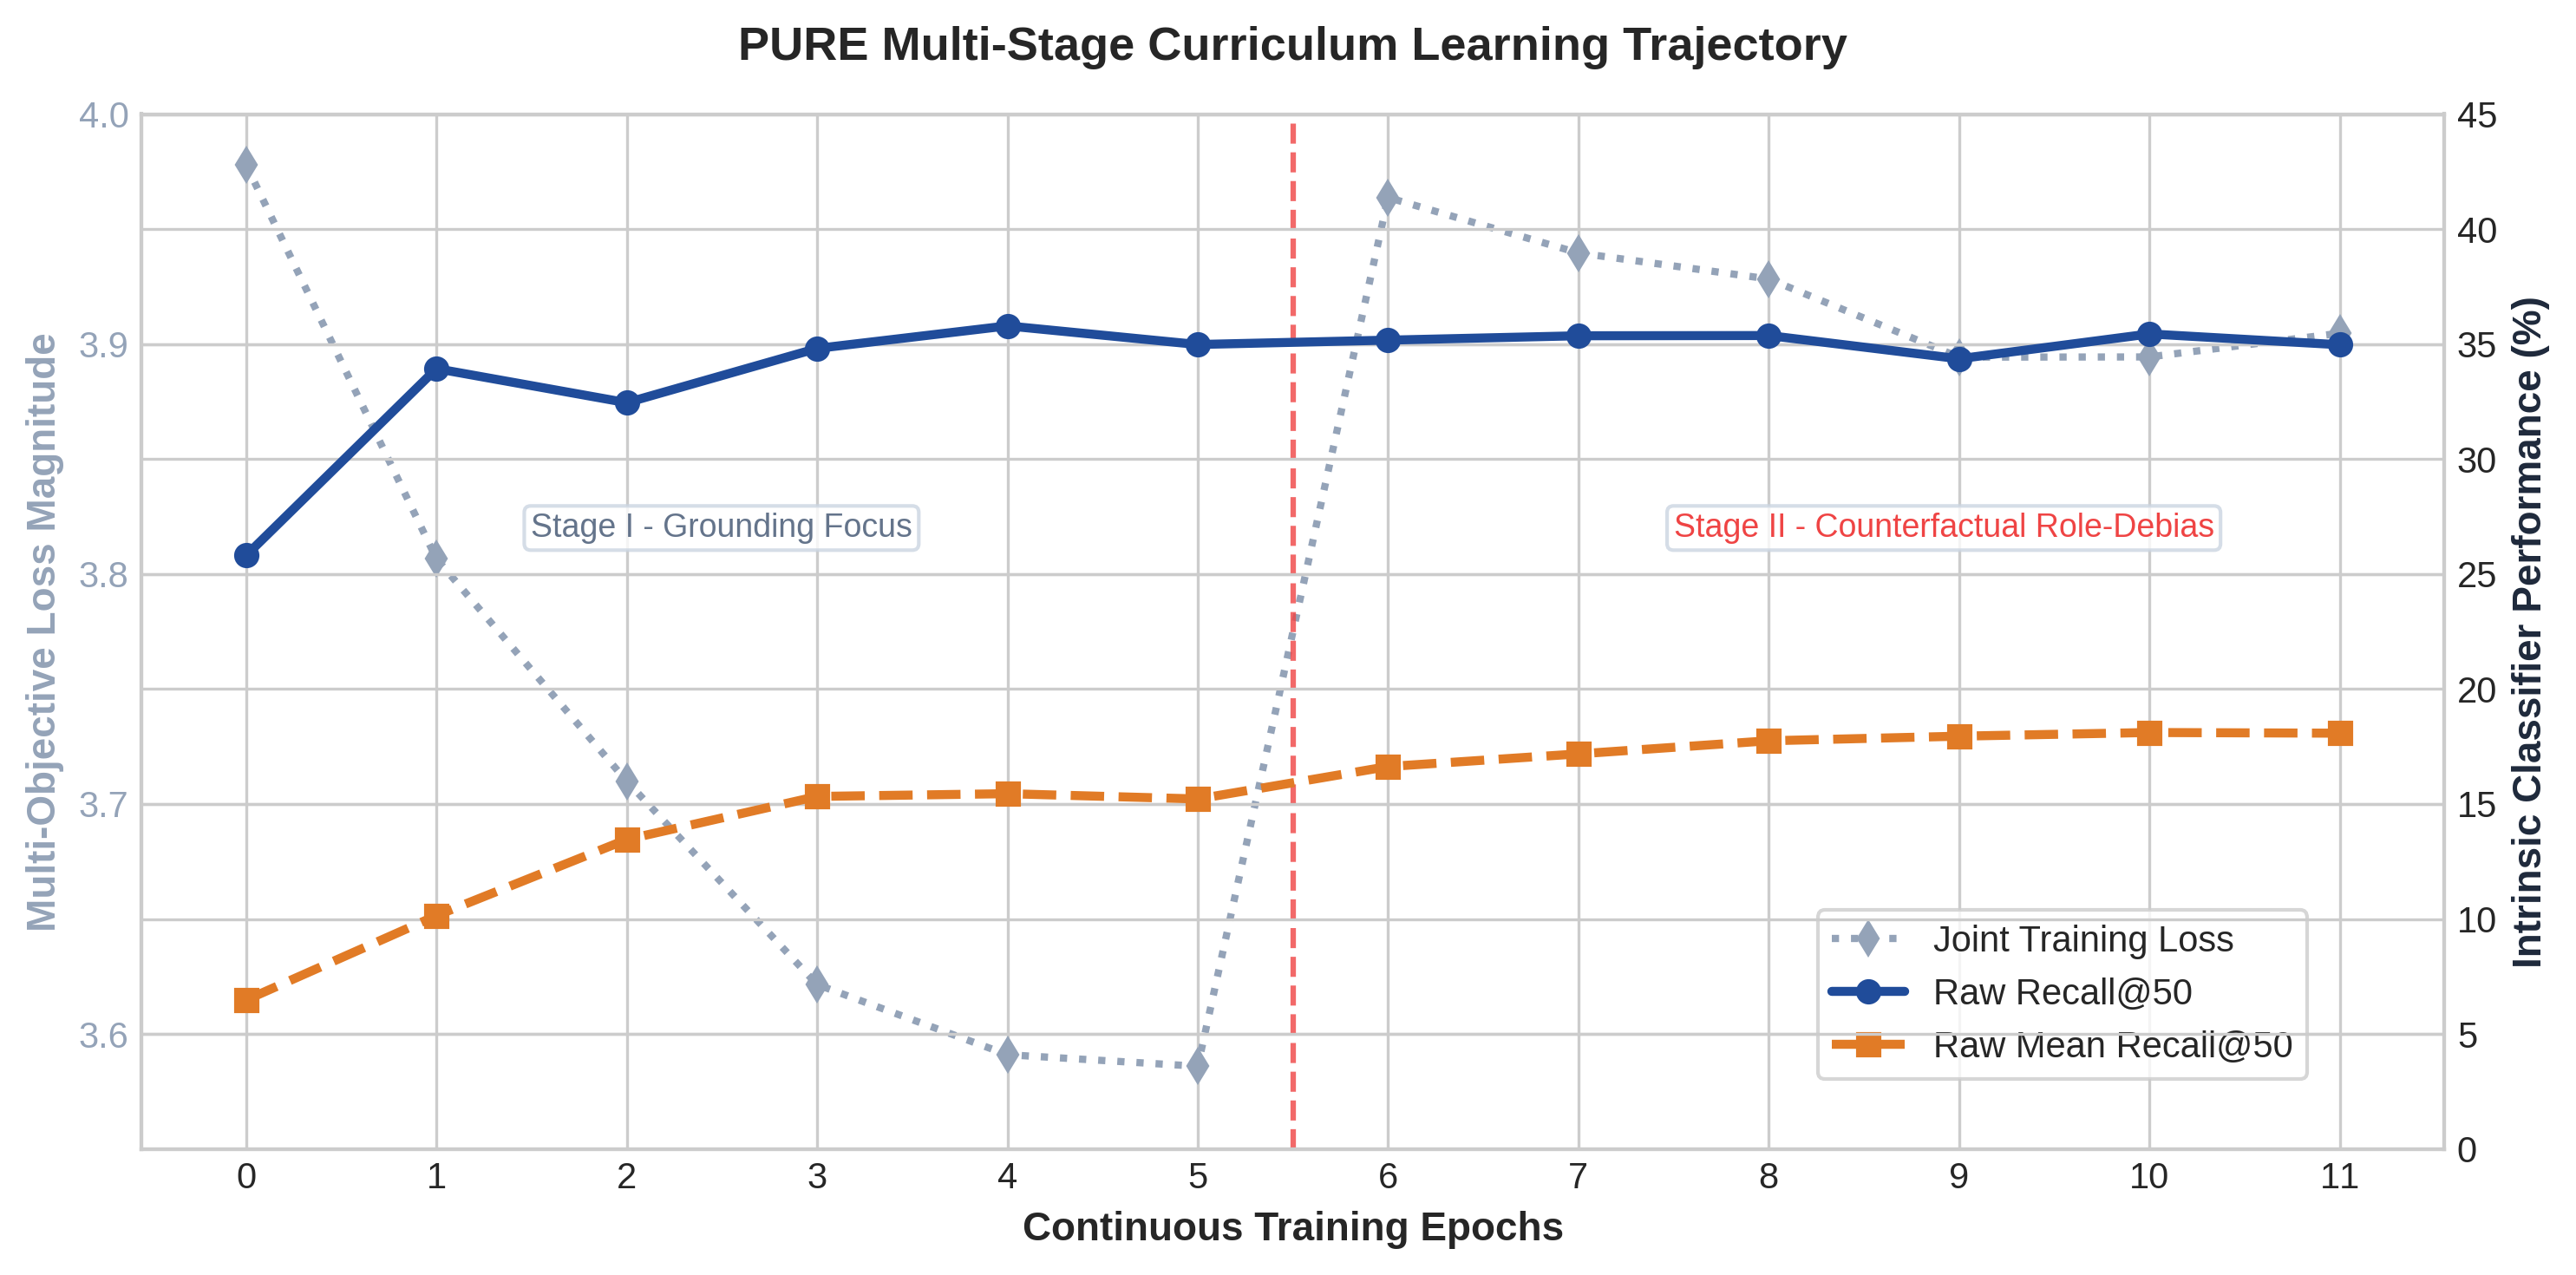
\includegraphics[width=\textwidth,height=0.70\textheight,keepaspectratio]{training_loss.png}
\source{Project training-loss plot; optimization context follows \href{https://arxiv.org/abs/2103.00020}{CLIP} fine-tuning practice.}
\end{frame}


\subsection{Calibration and Ablations}

\begin{frame}{Calibration Strength Sweep}

The sweep shows why calibration must be reported explicitly: the best raw tail score and best calibrated system score are different operating points.

\slidebody
\begin{table}[htbp]
\centering
\tablesize
\begin{tabular}{p{30mm} c c p{42mm}}
\toprule
\textbf{Calibration setting} & \textbf{R@50} & \textbf{mR@50} & \textbf{Reading} \\
\midrule
Adapt-light raw & 19.95 & \textbf{23.04} & High tail evidence, low aggregate. \\
Adapt-light fa10 & 62.55 & 19.33 & R@50 begins to recover. \\
Adapt-light fa225 & 66.15 & 22.03 & Balanced calibrated point. \\
Adapt-light fa375 & 67.09 & \textbf{22.99} & Best calibrated mR@50. \\
Adapt-light fa45 & \textbf{67.20} & 22.74 & Best R@50. \\
\bottomrule
\end{tabular}
\end{table}

\source{Project calibration sweep; long-tail calibration context: \href{https://openaccess.thecvf.com/content_cvpr_2020/html/Tang_Unbiased_Scene_Graph_Generation_From_Biased_Training_CVPR_2020_paper.html}{TDE}.}
\end{frame}


\begin{frame}{Calibration Plot}
\slidebody
{\slidesmall The calibration plot visualizes the raw-versus-calibrated trade-off: aggregate recall and mean recall peak at different operating points.}

\vspace{0.15em}
\centering
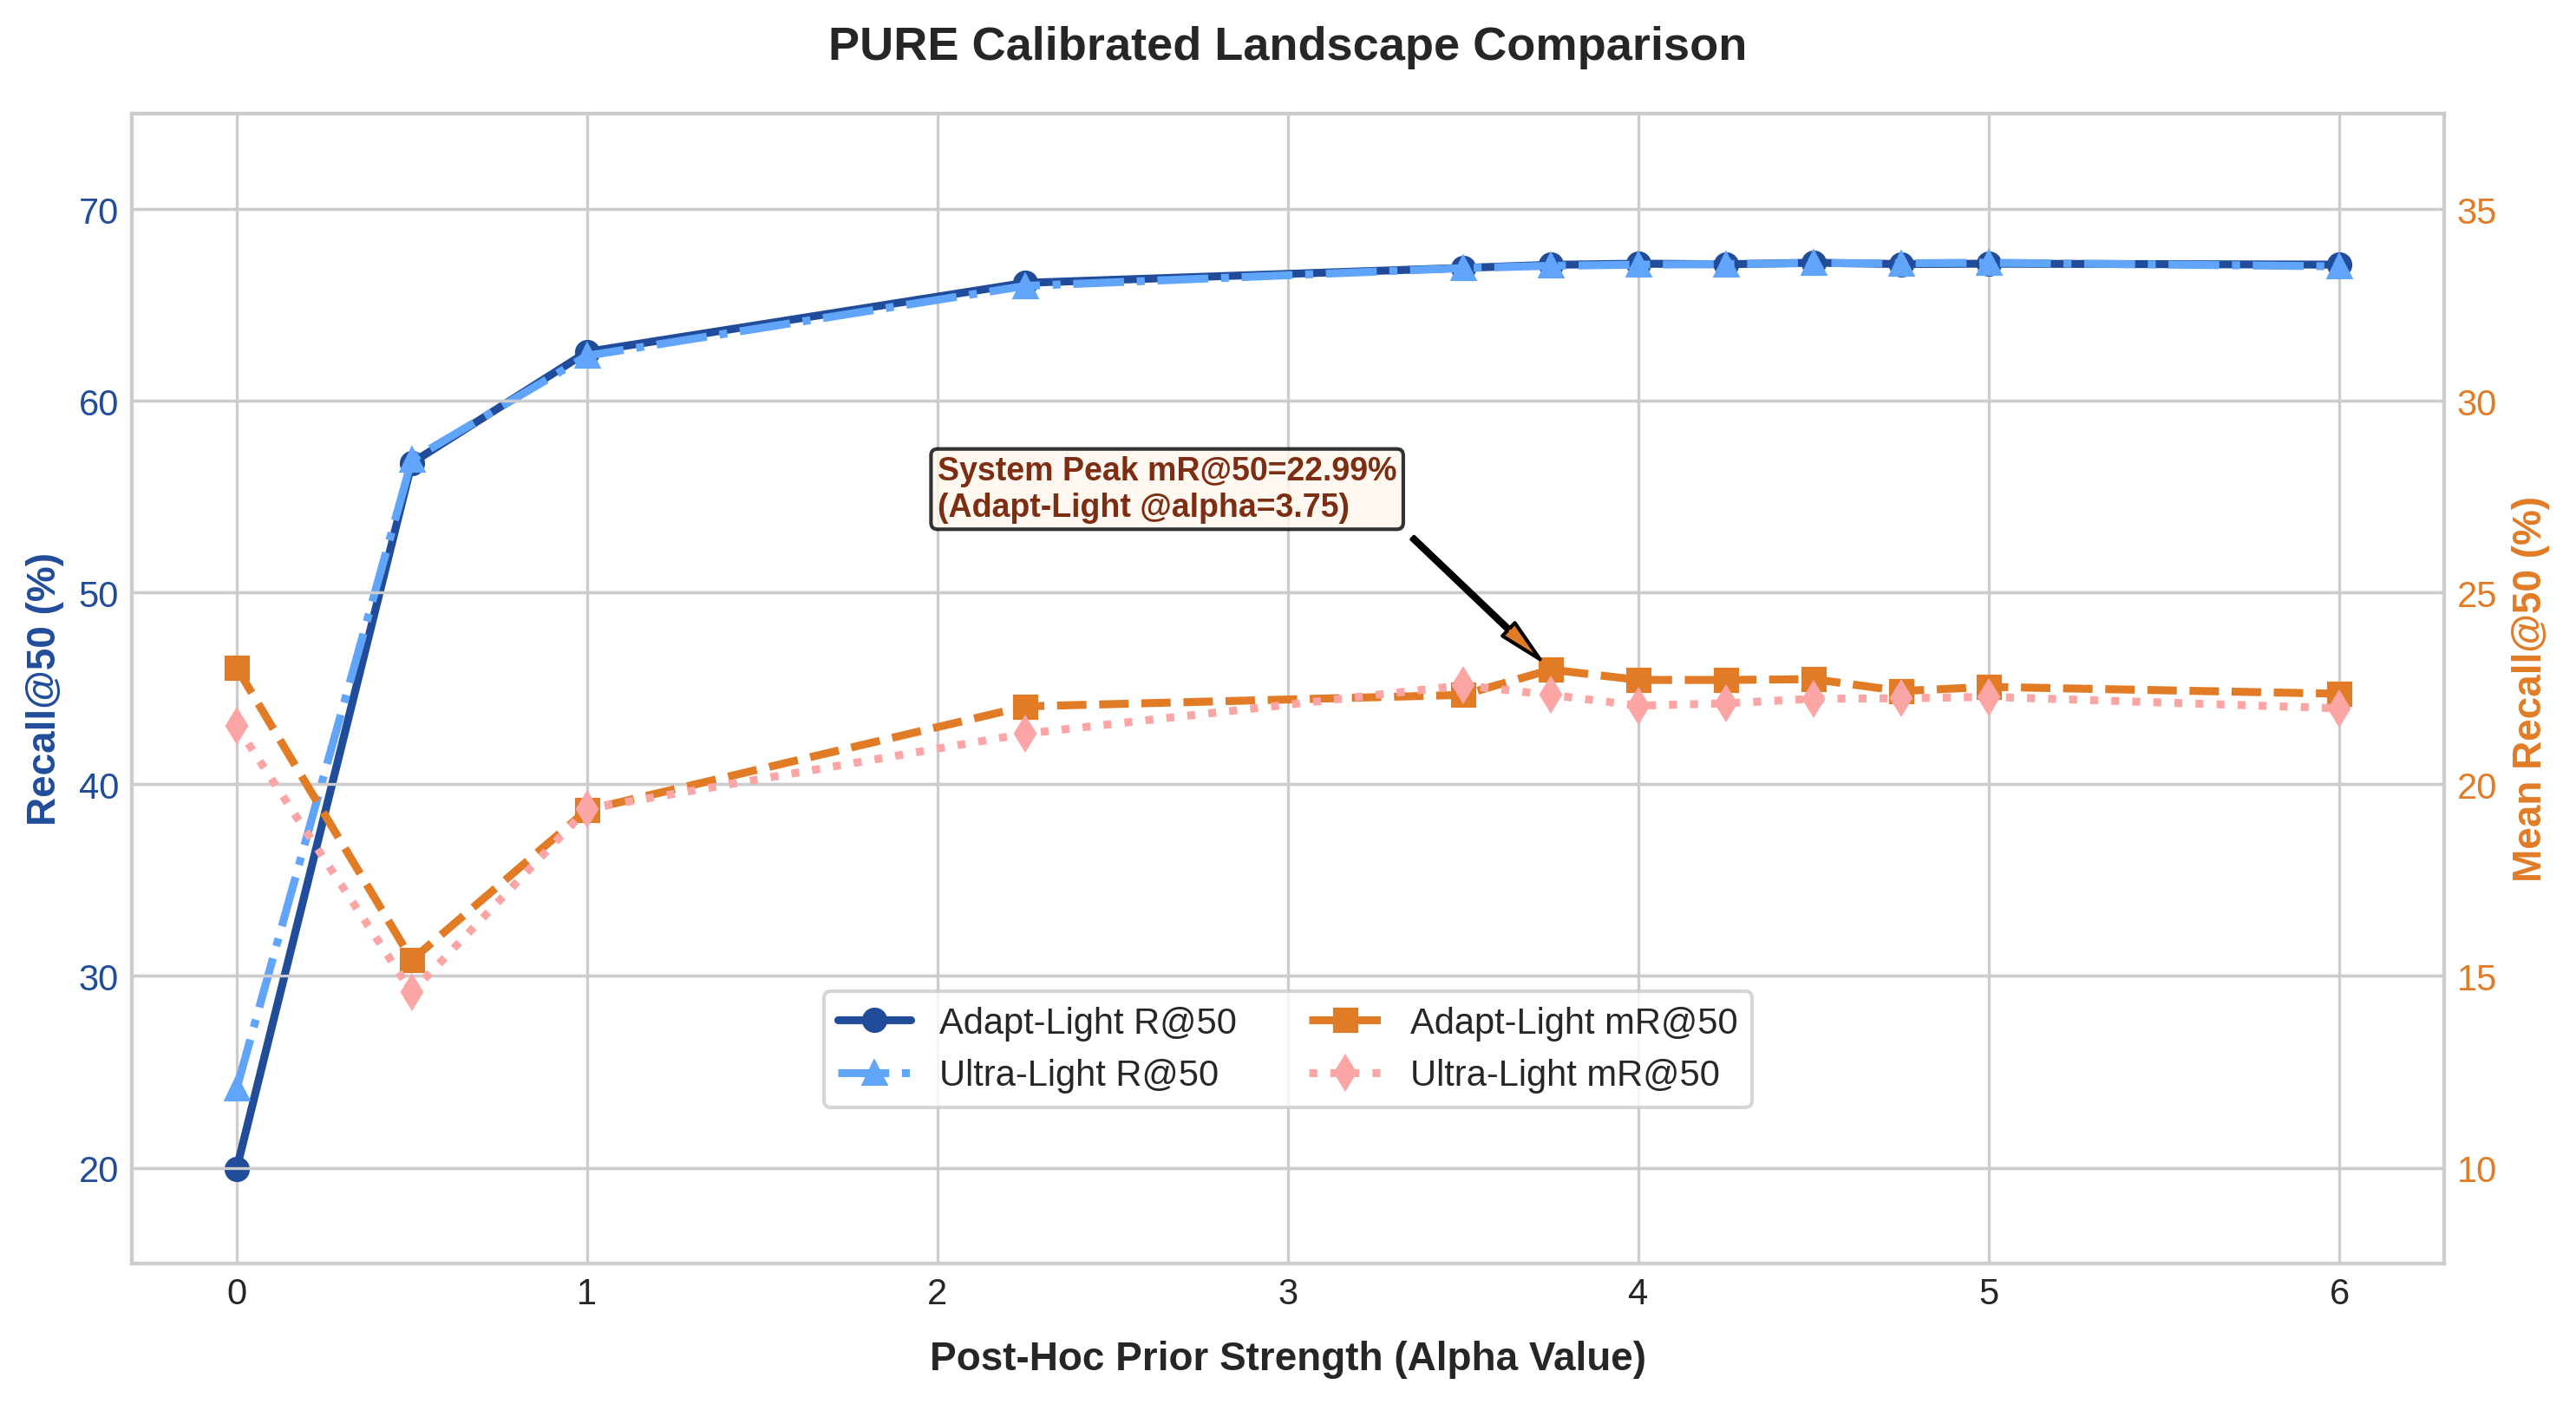
\includegraphics[width=\textwidth,height=0.70\textheight,keepaspectratio]{calibration.png}
\source{Project calibration plot; long-tail calibration context follows \href{https://openaccess.thecvf.com/content_cvpr_2020/html/Tang_Unbiased_Scene_Graph_Generation_From_Biased_Training_CVPR_2020_paper.html}{TDE}.}
\end{frame}

\begin{frame}{Comparison with Related SGG Methods}
\slidebody

PURE is strong in aggregate recall, while specialized debiasing methods remain stronger on long-tail mean recall.

\begin{table}[htbp]
\centering
\tablesize
\begin{tabular}{p{32mm} c c p{47mm}}
\toprule
\textbf{Method} & \textbf{R@50} & \textbf{mR@50} & \textbf{Interpretation} \\
\midrule
\href{https://openaccess.thecvf.com/content/ICCV2023/html/Li_Compositional_Feature_Augmentation_for_Unbiased_Scene_Graph_Generation_ICCV_2023_paper.html}{Motifs + CFA} & 54.10 & \textbf{35.70} & Best long-tail reference. \\
\href{https://eccv.ecva.net/virtual/2024/poster/2253}{SBG} & 55.80 & 33.30 & Strong sample-level debiasing. \\
\href{https://openaccess.thecvf.com/content_cvpr_2020/html/Tang_Unbiased_Scene_Graph_Generation_From_Biased_Training_CVPR_2020_paper.html}{ResCAGCN + PUM} & N/A & 20.20 & Prior debiasing reference. \\
\midrule
\textbf{PURE fa45} & \textbf{67.20} & 22.74 & Highest aggregate recall. \\
\textbf{PURE fa375} & 67.09 & 22.99 & Highest PURE mean recall. \\
\bottomrule
\end{tabular}
\end{table}


\source{External baselines: \href{https://openaccess.thecvf.com/content/ICCV2023/html/Li_Compositional_Feature_Augmentation_for_Unbiased_Scene_Graph_Generation_ICCV_2023_paper.html}{CFA}, \href{https://eccv.ecva.net/virtual/2024/poster/2253}{SBG}, \href{https://openaccess.thecvf.com/content_cvpr_2020/html/Tang_Unbiased_Scene_Graph_Generation_From_Biased_Training_CVPR_2020_paper.html}{TDE/PUM}. PURE: project logs.}
\end{frame}

\begin{frame}{Loss Component Ablation}
\slidebody

Removing grounding increases aggregate recall but lowers mR@50, suggesting that dense grounding helps protect tail predicates from head-prior domination.

\begin{table}[htbp]
\centering
\footnotesize
\begin{tabular}{p{30mm} c c c p{48mm}}
\toprule
\textbf{Setting} & \textbf{R@50} & \textbf{mR@50} & \textbf{$\Delta$mR} & \textbf{Reading} \\
\midrule
Full objective & 21.17 & \textbf{22.20} & N/A & Best head-tail balance. \\
Without SPOA & 21.39 & 21.41 & -0.79 & Mild tail degradation. \\
Without grounding & \textbf{28.36} & 19.11 & -3.09 & Head-prior spike; tail collapse. \\
\bottomrule
\end{tabular}
\end{table}


\source{Project loss-ablation logs; SGG protocol follows \href{https://openaccess.thecvf.com/content_cvpr_2018/html/Zellers_Neural_Motifs_Scene_CVPR_2018_paper.html}{Neural Motifs}.}
\end{frame}


\subsection{Retrieval Diagnostics}

\begin{frame}[fragile,shrink=4]{CORE Metadata}

\vspace{0.5em}
\begin{columns}[T]
    \begin{column}{0.0\textwidth}
    \end{column}
    % Cột 1: Hiển thị duy nhất Ảnh, được căn trái gọn gàng
    \begin{column}{0.37\textwidth}
        \vspace*{0pt}
        \centering
        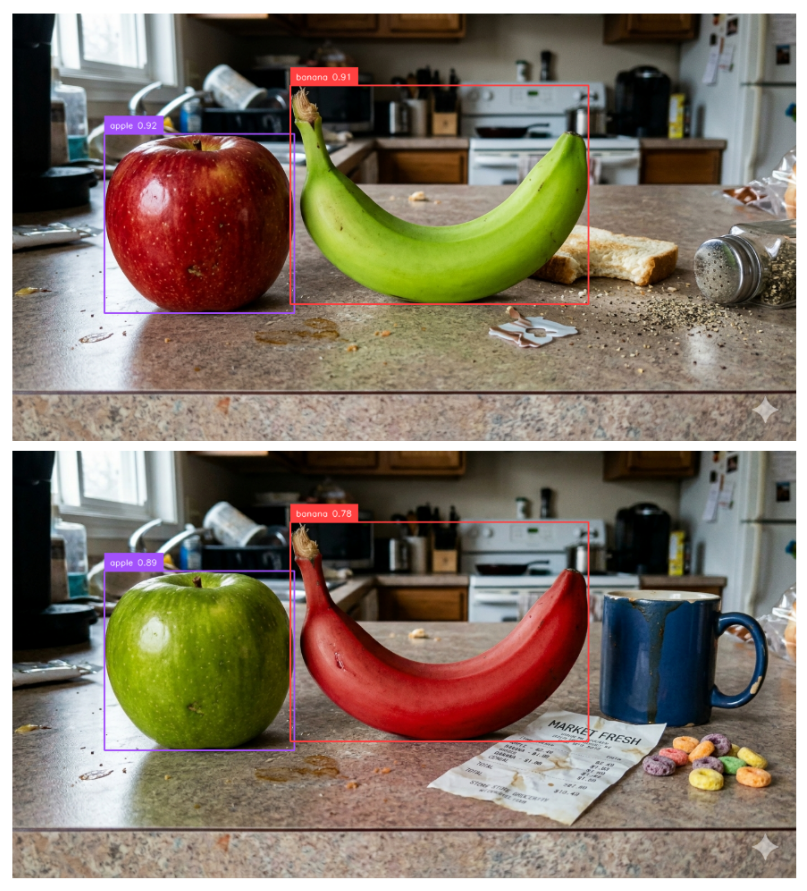
\includegraphics[width=\textwidth,keepaspectratio]{core_sample.png}
    \end{column}

    % Cột 2: Toàn bộ JSON (Chiếm không gian lớn hơn để tránh tràn dòng)
    \begin{column}{0.60\textwidth}
        \vspace*{0pt}
        \vspace*{-1.2em} % Kéo Verbatim lên để ngoặc nhọn { gióng bằng mép trên của ảnh
        \fontsize{6.2pt}{7.0pt}\selectfont
\begin{verbatim}
{
  "id": "Attribute_Binding_002",
  "type": "attribute_binding",
  "entities": {
    "e1": "apple",
    "e2": "banana"
  },
  "scene_A": {
    "caption": "A red apple is next to a green banana.",
    "attrs": {
      "e1": "red",
      "e2": "green"
    },
    "image": "Attribute_Binding_002_A.jpg",
    "boxes": {
      "e1": [0.239, 0.492, 0.243, 0.419],
      "e2": [0.545, 0.424, 0.380, 0.512]
    }
  },
  "scene_B": {
    "caption": "A green apple is next to a red banana.",
    "attrs": {
      "e1": "green",
      "e2": "red"
    },
    "image": "Attribute_Binding_002_B.jpg",
    "boxes": {
      "e1": [0.239, 0.492, 0.243, 0.419],
      "e2": [0.545, 0.424, 0.380, 0.513]
    }
  }
}
\end{verbatim}
    \end{column}

\end{columns}
\end{frame}

\begin{frame}{CORE Retrieval Diagnostics}
\slidebody
CORE retrieval diagnostics should be read together with coverage because each group stresses a different relation skill.

\begin{table}[htbp]
\centering
\tablesize
\begin{tabular}{p{45mm} c c c p{40mm}}
\toprule
\textbf{CORE group} & \textbf{Acc.} & \textbf{Cov.} & \textbf{N} & \textbf{Reading} \\
\midrule
VG-compatible boxed retrieval & \textbf{0.591} & 0.603 & 2045 & Moderate transfer. \\
Attribute Binding, text-image & 0.518 & 1.000 & 280 & Best hybrid text cue. \\
Gaze-Attention & 0.597 & 0.702 & 442 & Stronger gaze transfer. \\
Occlusion-Depth & 0.490 & 0.844 & 437 & Depth direction is hard. \\
Spatial-Containment & 0.612 & 0.724 & 343 & Strongest reliable group. \\
Extreme Compositional OOD & 0.710 & 0.246 & 31 & High score, limited coverage. \\
Action-Role, text triplet & 0.538 & 1.000 & 478 & Weak role sensitivity. \\
\bottomrule
\end{tabular}
\end{table}

\source{Project CORE retrieval logs; compositional evaluation reference: \href{https://arxiv.org/abs/2212.09645}{SugarCrepe}.}
\end{frame}

\begin{frame}[shrink=6]{Qualitative Result: "man riding horse"}
\slidebody
This qualitative case shows the intended retrieval-facing output: predicted relation triplets can be inspected directly for a text query such as ``man riding horse''.

\vspace{0.15em}
\centering
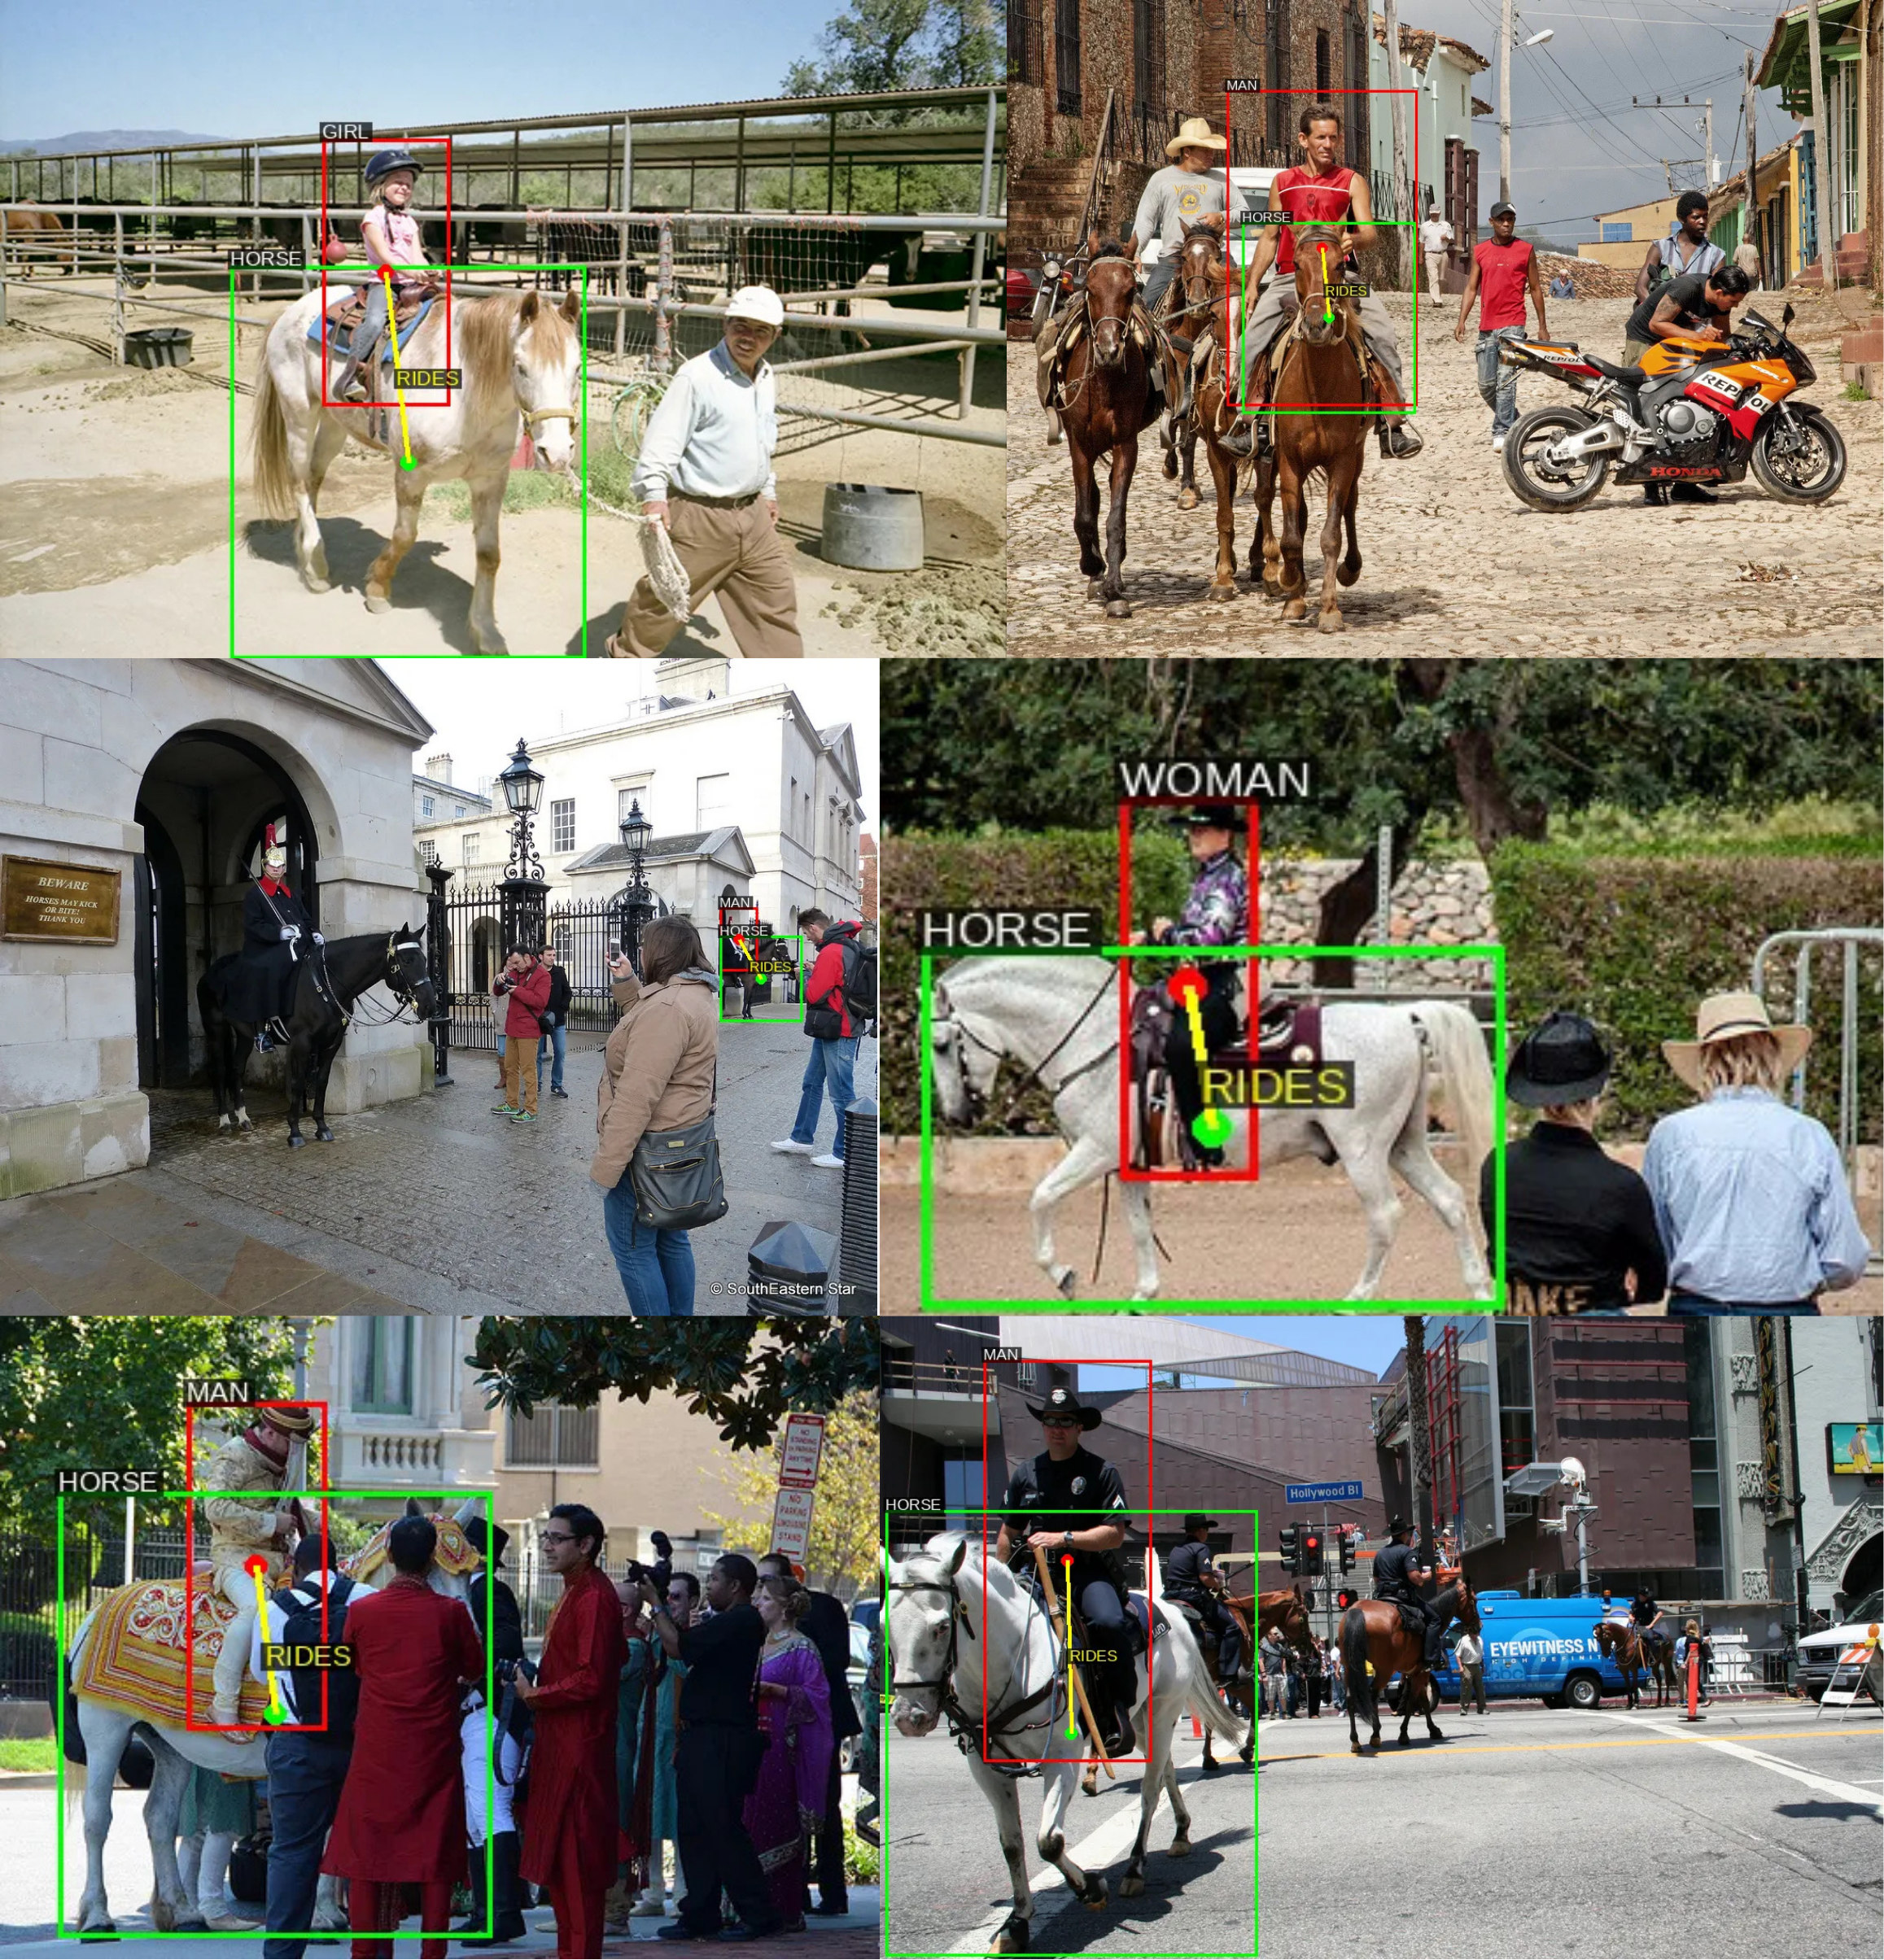
\includegraphics[width=0.96\textwidth,height=0.72\textheight,keepaspectratio]{horse.png}
\source{Project qualitative prediction example; retrieval motivation follows \href{https://openaccess.thecvf.com/content/CVPR2022/papers/Li_SGTR_End-to-End_Scene_Graph_Generation_With_Transformer_CVPR_2022_paper.pdf}{SGTR}.}
\end{frame}

% =============================================================================
\section{Conclusion}
\subsection{Summary and Future Work}


\begin{frame}{Conclusion}
\slidebody
\begin{talert}{Model implementation}
\begin{enumerate}
  \item Implemented PURE as a compact directed-pair predicate scorer with dense CLIP evidence and object routing.
  \item Added asymmetric SPOA relation states, progressive relation refinement, text/classifier scoring, relationness, and calibration readouts.
  \item Trained and evaluated under a reproducible L4 24GB configuration.
\end{enumerate}
\end{talert}

\source{Summary based on project implementation and experimental logs; protocol context follows \href{https://openaccess.thecvf.com/content_cvpr_2018/html/Zellers_Neural_Motifs_Scene_CVPR_2018_paper.html}{Neural Motifs}.}

\slidebody
\begin{talert}{Empirical outcomes}
\begin{enumerate}
  \item Reported VG150 PredCls with both R@50 and mR@50, separating raw and calibrated scores.
  \item Built CORE examples and retrieval diagnostics for role, attribute, spatial, gaze, occlusion, and OOD cases.
  \item Demonstrated relation-aware retrieval with predicted triplets such as \triplet{man}{ride}{horse}.
\end{enumerate}
\end{talert}

\source{Summary based on VG150 logs, CORE diagnostics, and qualitative predictions; compositional context follows \href{https://arxiv.org/abs/2212.09645}{SugarCrepe}.}
\end{frame}

\begin{frame}{Limitations and Future Work}

\slidebody
\begin{talert}{Limitations}
\begin{enumerate}
  \item Grounding--bias trade-off: stronger grounding and calibration can improve tail-class fairness but may reduce aggregate R@50.
  \item Static-image scope: the current system does not model temporal dynamics for video-based actions.
\end{enumerate}
\end{talert}

\source{Summary based on project implementation and experimental logs; long-tail context follows \href{https://openaccess.thecvf.com/content_cvpr_2020/html/Tang_Unbiased_Scene_Graph_Generation_From_Biased_Training_CVPR_2020_paper.html}{TDE}.}

\slidebody
\begin{talert}{Future works}
\begin{enumerate}
  \item Improve long-tail mR@50 with stronger debiasing and sample-level training.
  \item Replace fixed calibration sweeps with constrained learnable calibration.
  \item Extend object-label prediction for SGCls and SGDet settings.
  \item Expand CORE vocabulary, audits, and retrieval demo coverage.
  \item Explore 3D and video SGG after the 2D relation protocol is stable.
\end{enumerate}
\end{talert}

\source{Future directions informed by \href{https://openaccess.thecvf.com/content/ICCV2023/html/Li_Compositional_Feature_Augmentation_for_Unbiased_Scene_Graph_Generation_ICCV_2023_paper.html}{CFA}, \href{https://eccv.ecva.net/virtual/2024/poster/2253}{SBG}, \href{https://openaccess.thecvf.com/content/CVPR2022/papers/Li_SGTR_End-to-End_Scene_Graph_Generation_With_Transformer_CVPR_2022_paper.pdf}{SGTR}, and the report conclusion.}
\end{frame}

\begin{frame}{Retrieval Demo}
\slidebody
A user enters a relation query such as ``man ride horse''. The system matches the query against predicted triplets and returns images ranked by relation agreement.

\vspace{0.15em}
\centering

\includegraphics[width=\textwidth,height=0.70\textheight,keepaspectratio]{pics/qrcode.png}%

\vspace{0.5em}

\source{Retrieval application follows the SGG-to-structured-query motivation in \href{https://openaccess.thecvf.com/content/CVPR2022/papers/Li_SGTR_End-to-End_Scene_Graph_Generation_With_Transformer_CVPR_2022_paper.pdf}{SGTR}.}
\end{frame}

\begin{frame}{References I}
\footnotesize
\begin{enumerate}
  \item \href{https://link.springer.com/article/10.1007/s11263-016-0981-7}{Krishna et al., ``Visual Genome: Connecting Language and Vision Using Crowdsourced Dense Image Annotations,'' IJCV 2017.}
  \item \href{https://arxiv.org/abs/2103.00020}{Radford et al., ``Learning Transferable Visual Models From Natural Language Supervision,'' ICML 2021.}
  \item \href{https://openaccess.thecvf.com/content_cvpr_2018/html/Zellers_Neural_Motifs_Scene_CVPR_2018_paper.html}{Zellers et al., ``Neural Motifs: Scene Graph Parsing with Global Context,'' CVPR 2018.}
  \item \href{https://openaccess.thecvf.com/content/CVPR2022/papers/Li_SGTR_End-to-End_Scene_Graph_Generation_With_Transformer_CVPR_2022_paper.pdf}{Li et al., ``SGTR: End-to-End Scene Graph Generation With Transformer,'' CVPR 2022.}
  \item \href{https://openaccess.thecvf.com/content_cvpr_2020/html/Tang_Unbiased_Scene_Graph_Generation_From_Biased_Training_CVPR_2020_paper.html}{Tang et al., ``Unbiased Scene Graph Generation from Biased Training,'' CVPR 2020.}
  \item \href{https://openaccess.thecvf.com/content/ICCV2023/html/Li_Compositional_Feature_Augmentation_for_Unbiased_Scene_Graph_Generation_ICCV_2023_paper.html}{Li et al., ``Compositional Feature Augmentation for Unbiased Scene Graph Generation,'' ICCV 2023.}
  \item \href{https://eccv.ecva.net/virtual/2024/poster/2253}{Li et al., ``Fine-Grained Scene Graph Generation via Sample-Level Bias Prediction,'' ECCV 2024.}
  \item \href{https://openaccess.thecvf.com/content_cvpr_2017/html/Xu_Scene_Graph_Generation_CVPR_2017_paper.html}{Xu et al., ``Scene Graph Generation by Iterative Message Passing,'' CVPR 2017.}
  \item \href{https://openaccess.thecvf.com/content_CVPR_2019/html/Tang_Learning_to_Compose_Dynamic_Tree_Structures_for_Visual_Contexts_CVPR_2019_paper.html}{Tang et al., ``Learning to Compose Dynamic Tree Structures for Visual Contexts,'' CVPR 2019.}
  \item \href{https://arxiv.org/abs/2201.11460}{Cong et al., ``RelTR: Relation Transformer for Scene Graph Generation,'' arXiv 2022.}
\end{enumerate}
\end{frame}

\begin{frame}{References II}
\footnotesize
\begin{enumerate}
  \setcounter{enumi}{10}
  \item \href{https://arxiv.org/abs/2212.09645}{Hsieh et al., ``SugarCrepe: Fixing Hackable Benchmarks for Vision-Language Compositionality,'' NeurIPS 2023.}
  \item \href{https://arxiv.org/abs/2303.05499}{Liu et al., ``Grounding DINO: Marrying DINO with Grounded Pre-Training for Open-Set Object Detection,'' arXiv 2023.}
  \item \href{https://arxiv.org/abs/2404.00906}{Yao et al., ``From Pixels to Graphs: Open-Vocabulary Scene Graph Generation with Vision-Language Models,'' CVPR 2024.}
  \item \href{https://arxiv.org/abs/2306.05424}{Lai et al., ``LISA: Reasoning Segmentation via Large Language Model,'' arXiv 2023.}
  \item \href{https://arxiv.org/abs/2304.02643}{Zou et al., ``Segment Everything Everywhere All at Once,'' NeurIPS 2023.}
  \item \href{https://arxiv.org/abs/2405.14458}{OpenAI, ``GPT-4o System Card,'' 2024.}
\end{enumerate}
\end{frame}

\standout{Thank you!}

\end{document}